\documentclass[11pt,a4paper]{article}
\usepackage[utf8]{inputenc}
\usepackage[T1]{fontenc}
\usepackage[brazil]{babel}
\usepackage[margin=2.3cm]{geometry}
\usepackage{booktabs}
\usepackage{amsmath,amssymb}
\usepackage{caption}
\usepackage{graphicx}
\usepackage{setspace}
\usepackage{enumitem}
\usepackage{xcolor}
\usepackage{placeins}
\usepackage{longtable}
\usepackage{float}
\usepackage[hidelinks]{hyperref}
\graphicspath{{figuras/}}
\definecolor{azul}{RGB}{20,60,110}
\definecolor{verde}{RGB}{20,110,70}
\definecolor{vermelho}{RGB}{150,30,30}
\newcommand{\pergunta}[1]{\par\vspace{4pt}\noindent\textbf{\color{azul}A pergunta:} #1\par\vspace{2pt}}
\newcommand{\equacao}[0]{\par\vspace{4pt}\noindent\textbf{\color{vermelho}A equação estimada:}\ }
\newcommand{\aha}[1]{\par\vspace{4pt}\noindent\textbf{\color{vermelho}Achado:} #1\par\vspace{2pt}}
\emergencystretch=2.5em
\setstretch{1.15}
\captionsetup{font=small,labelsep=colon}
\setcounter{tocdepth}{2}

\title{\textbf{v2 OFICIAL}\\[8pt]
\Large Peso de VALE3 nos fundos do Itaú --- versão simples, direta e objetiva\\[4pt]
\normalsize Cross-section (MQO + logit), ajuste parcial e um esquema in/out-of-sample ---
sem Newey--West, sem Kalman, sem Diebold--Mariano, sem múltiplos métodos de robustez}
\author{João Paulo Zangrandi (FGV--EESP)}
\date{}

\begin{document}
\maketitle

\begin{abstract}
\noindent Este documento retoma o projeto a partir da ideia original das anotações do
orientador: uma cross-section simples que estima um fator latente $\theta$, uma etapa
logística para manter a previsão dentro de $[0,1]$, e um modelo de ajuste parcial para a
dinâmica. Cada etapa usa \textbf{um único método} (MQO ou MQO logístico), sem testes ou
correções de robustez em cascata. Nesta versão, as características do fundo (inclusive o novo
beta do próprio fundo) passam a ser sempre medidas no \textbf{último dia do mês anterior},
eliminando qualquer look-ahead bias.
\end{abstract}

\newpage
\tableofcontents
\newpage

% ======================================================================
\section{Por que esta versão existe}

As versões anteriores deste projeto acumularam camada sobre camada de robustez estatística
(Newey--West, filtro de Kalman, variável instrumental com múltiplos esquemas de cluster,
painel dinâmico de Arellano--Bond, teste de Diebold--Mariano) até o núcleo do modelo ficar
difícil de enxergar por trás das correções. Esta versão volta ao desenho original discutido
com o orientador: uma cross-section por mínimos quadrados que gera um fator latente $\theta$,
uma etapa logística (a única forma de robustez mantida, porque o peso é limitado a $[0,1]$ e a
reta não respeita esse limite), e um modelo de ajuste parcial estimado diretamente por MQO. Cada
etapa produz um erro, examinado com estatísticas simples --- média, desvio-padrão, assimetria,
curtose, histograma --- sem bateria de testes formais.

A base de dados (composição de carteiras da CVM, fundos do grupo Itaú, 2016--2021) é a mesma já
construída e validada na versão anterior --- essa parte nunca foi a fonte da complexidade.

% ======================================================================
\FloatBarrier
\section{Etapa 1: a cross-section (MQO + logit)}
\label{sec:etapa1}

\pergunta{As características de um fundo explicam o peso de VALE3 que ele carrega? E, se sim,
como transformar essa explicação numa previsão que respeite os limites de $0\%$ a $100\%$?}

Esta etapa une o que em versões anteriores deste documento eram duas seções separadas: a
cross-section \textbf{linear} (para interpretar os coeficientes diretamente em pontos
percentuais) e a cross-section \textbf{logística} (para gerar um peso previsto que nunca sai de
$[0,1]$). As duas usam as mesmas cinco características, mês a mês:

\equacao
\begin{align}
\text{peso}_{i,t} &= \alpha_t + \theta^{aum}_t z(\ln AUM_{i}) + \theta^{cot}_t z(\ln\text{cot}_{i})
  + \theta^{fic}_t FIC_i + \theta^{flow}_t\Big(\tfrac{\text{capt}-\text{resg}}{AUM}\Big)_i
  + \theta^{bf}_t z(\beta^{fundo}_i) + \text{erro}_{i,t} \label{eq:cs}\\[4pt]
\text{peso}_{i,t} &= g\big(x_{i,t}'\theta_t\big) + e_{i,t}, \qquad g(z)=\frac{1}{1+e^{-z}}
\label{eq:logit}
\end{align}
$\theta_t=(\alpha_t,\theta^{aum}_t,\theta^{cot}_t,\theta^{fic}_t,\theta^{flow}_t,\theta^{bf}_t)$
é o vetor de coeficientes de \textbf{um único mês} $t$; $\Theta=\{\theta_t\}_{t}$, o \textbf{teta
grande}, é o conjunto de todos os $\theta_t$ ao longo do tempo --- é esse conjunto que as tabelas
e figuras a seguir resumem (média, desvio-padrão, evolução mês a mês).

A primeira é estimada por MQO (coeficientes em pontos percentuais, fáceis de interpretar); a
segunda por máxima verossimilhança (\texttt{glm} quase-binomial), a única forma de robustez
mantida nesta versão, porque $x'\theta$ pode sair de $[0,1]$ mas $g(x'\theta)$ nunca sai. As
duas rodam mês a mês, uma regressão por mês, sem nenhuma etapa de resumo temporal em cima
(não é Fama--MacBeth).

\textbf{Novidade desta versão --- duas mudanças na Etapa 1:}
\begin{enumerate}[topsep=2pt,itemsep=2pt]
\item[(a)] Entra uma 5ª característica, o \textbf{beta do próprio fundo} $\beta^{fundo}$: mede o
quanto a cota do fundo se move junto com o mercado (Ibovespa), do mesmo jeito que se mede o beta
de uma ação.
\equacao
$$r_{i,d} = \frac{\text{cota}_{i,d}}{\text{cota}_{i,d-1}} - 1 \qquad\qquad
r_{m,d} = \frac{\text{Ibov}_d}{\text{Ibov}_{d-1}} - 1$$
$$\beta^{fundo}_{i,t} = \frac{\widehat{\text{Cov}}_{252}\big(r_i,\,r_m\big)}
{\widehat{\text{Var}}_{252}\big(r_m\big)}$$
$r_{i,d}$ é o retorno diário da cota do fundo $i$; $r_{m,d}$ é o retorno diário do Ibovespa;
$\widehat{\text{Cov}}_{252}$ e $\widehat{\text{Var}}_{252}$ são covariância e variância amostrais
numa janela móvel dos últimos $252$ pregões (${\approx}1$ ano), terminando no último pregão do
mês $t-1$ --- mesma metodologia (e mesma janela) já usada para o beta de VALE3 (mercado) no
\texttt{tcc I.pdf} (v1), agora aplicada à \emph{cota do fundo} em vez do preço da ação.
\item[(b)] \textbf{Todas} as cinco características (não só o beta do fundo) passam a ser medidas
no \textbf{último dia do mês anterior} ($t-1$), nunca no mês corrente --- antes, $AUM$, cotistas
e fluxo eram contemporâneos ao próprio mês $t$. Agora $\theta_t$ é 100\% predeterminado: tudo que
ele usa já era conhecido antes do mês $t$ começar.
\end{enumerate}

\textbf{Adendo sobre a amostra:} exigir as cinco características simultaneamente reduz a
cobertura de 72 para \textbf{59 meses} (fev/2017 a dez/2021) --- o beta do fundo exige
$\geq252$ pregões de histórico de cota (quase um ano), então nenhum fundo tem essa variável
disponível nos primeiros meses da amostra (jan/2016 a jan/2017 ficam sem fundos suficientes).
Essa perda foi aceita conscientemente, não é um erro: a partir daqui, todo número deste
documento vem dos $8.335$ fundo-meses com as cinco características completas ($120$ a $190$
fundos por mês, média $141$).

\subsection{O resultado: antes e depois do beta do fundo}

Para deixar claro o efeito de adicionar o beta do fundo, a tabela abaixo compara --- na
\textbf{mesma amostra} de $59$ meses --- a regressão \textbf{logística} (equação~\eqref{eq:logit},
a que de fato alimenta o erro $e$ e todo o resto do documento a partir daqui) com as quatro
características clássicas contra a mesma regressão com o beta do fundo incluído. Os coeficientes
estão na escala do preditor linear $x'\theta$ (log-odds), não em pontos percentuais.

\begin{table}[h]\centering\small
\caption{$\Theta$ logístico: antes e depois do beta do fundo (mesma amostra, 59 meses, teste
ingênuo de significância $t=\bar\theta/(\text{dp}(\theta)/\sqrt{59})$).}
\begin{tabular}{@{}lrcrc@{}}
\toprule
Variável & Média (sem $\beta^{fundo}$) & Sig. & Média (com $\beta^{fundo}$) & Sig. \\
\midrule
$\alpha$                   & $-3{,}1262$ & *** & $-3{,}8110$ & *** \\
$\theta^{aum}$ (tamanho)        & $-0{,}2749$ & *** & $-0{,}0594$ & *** \\
$\theta^{cot}$ (cotistas)       & $0{,}4429$  & *** & $0{,}0493$  & *** \\
$\theta^{fic}$ (fundo de cotas) & $-0{,}6669$ & *** & $-0{,}2149$ & *** \\
$\theta^{flow}$ (captação/resgate) & $0{,}4402$ & n.s. & $0{,}1396$ & n.s. \\
$\theta^{bf}$ (beta do fundo)   & ---          & ---& $1{,}0110$  & *** \\
\midrule
Pseudo-$R^2$ (McFadden) médio & $0{,}164$ & & $0{,}614$ & \\
\bottomrule
\end{tabular}
\caption*{\footnotesize $^{*}p<5\%$, $^{**}p<1\%$, $^{***}p<0{,}1\%$. Fonte: elaboração própria
(\texttt{scripts/13\_etapa1\_unificada.R}, \texttt{14\_etapa1\_antes\_depois.R}). \textbf{Nota de
correção:} uma versão anterior deste documento reportava $t$ errado nesta tabela (usava
$\sqrt{6}$, o número de \emph{variáveis}, em vez de $\sqrt{59}$, o número de \emph{meses}, no
denominador do teste) --- os $t$ corretos são $\approx3{,}1\times$ maiores; tamanho e cotistas
continuam *** significativos com o beta do fundo, não n.s./* como antes reportado.}
\end{table}

\aha{O mesmo padrão que já tinha aparecido como checagem à parte na versão anterior (Tabela 11
do \texttt{tcc I.pdf}) agora é a especificação principal: com o beta do fundo na conta, tamanho e
cotistas ficam \textbf{bem mais fracos} em magnitude de $t$ (tamanho: $t=-15{,}1\to-6{,}0$;
cotistas: $t=31{,}5\to4{,}9$) --- mas \textbf{continuam estatisticamente significativos a
$0{,}1\%$}, não perdem a significância. O pseudo-$R^2$ quase quadruplica
($0{,}164\to0{,}614$). Leitura: parte do que tamanho e cotistas explicavam era, na verdade, um
proxy indireto para o quão ``equity-like'' é o fundo --- o beta do fundo mede isso diretamente e
absorve boa parte (não toda) dessa força explicativa.}

\subsubsection*{Tornando o logit interpretável: efeito marginal médio}

Um coeficiente logístico não é ``pontos percentuais'' --- está na escala do preditor linear
$x'\theta$ (log-odds), não na escala do peso em si. Para interpretar em pontos percentuais sem
abandonar o logit, uso o \textbf{efeito marginal médio} (\emph{average partial effect}, APE):
para uma característica contínua $k$, $\text{APE}_k=\theta_k\cdot\overline{g'(x'\theta)}$, a média
(em toda a amostra) da inclinação de $g(\cdot)$ vezes o coeficiente --- quanto o peso previsto se
move, em média, para uma variação de $1$ desvio-padrão naquela característica. Para o FIC (0/1,
discreta), uso a diferença média de $g(\cdot)$ forçando FIC$=1$ contra FIC$=0$ em cada fundo,
mantendo as demais características observadas --- mais correto que a derivada para uma variável
que só assume dois valores.

\begin{table}[h]\centering\small
\caption{Efeito marginal médio (APE) do logit, em pontos percentuais de peso --- mesma
comparação sem/com beta do fundo.}
\begin{tabular}{@{}lrcrc@{}}
\toprule
Característica & APE (sem $\beta^{fundo}$) & Sig. & APE (com $\beta^{fundo}$) & Sig. \\
\midrule
Tamanho              & $-0{,}00734$ & *** & $-0{,}00154$ & *** \\
Cotistas             & $0{,}01271$  & *** & $0{,}00111$  & *** \\
Fundo de cotas       & $-0{,}02222$ & *** & $-0{,}00580$ & *** \\
Captação/resgate     & $0{,}01068$  & n.s. & $0{,}00449$ & n.s. \\
Beta do fundo        & ---           & --- & $0{,}02942$  & *** \\
\bottomrule
\end{tabular}
\caption*{\footnotesize Fonte: elaboração própria (\texttt{scripts/13\_etapa1\_unificada.R},
\texttt{14\_etapa1\_antes\_depois.R}).}
\end{table}

\aha{O APE bate de perto com o que a versão linear já dava (tamanho $-0{,}0074\to-0{,}0016$
linear vs.\ $-0{,}00734\to-0{,}00154$ via APE; cotistas $0{,}0130\to0{,}0018$ linear vs.\
$0{,}01271\to0{,}00111$ via APE) --- não é coincidência: quando o modelo se ajusta bem, a
inclinação média do logit converge para perto do coeficiente linear equivalente. A vantagem do
APE é que ele vem do \textbf{próprio} modelo logístico (respeitando os limites de $[0,1]$), não
de uma regressão linear separada rodada só para efeito de leitura.}

\begin{figure}[h]\centering
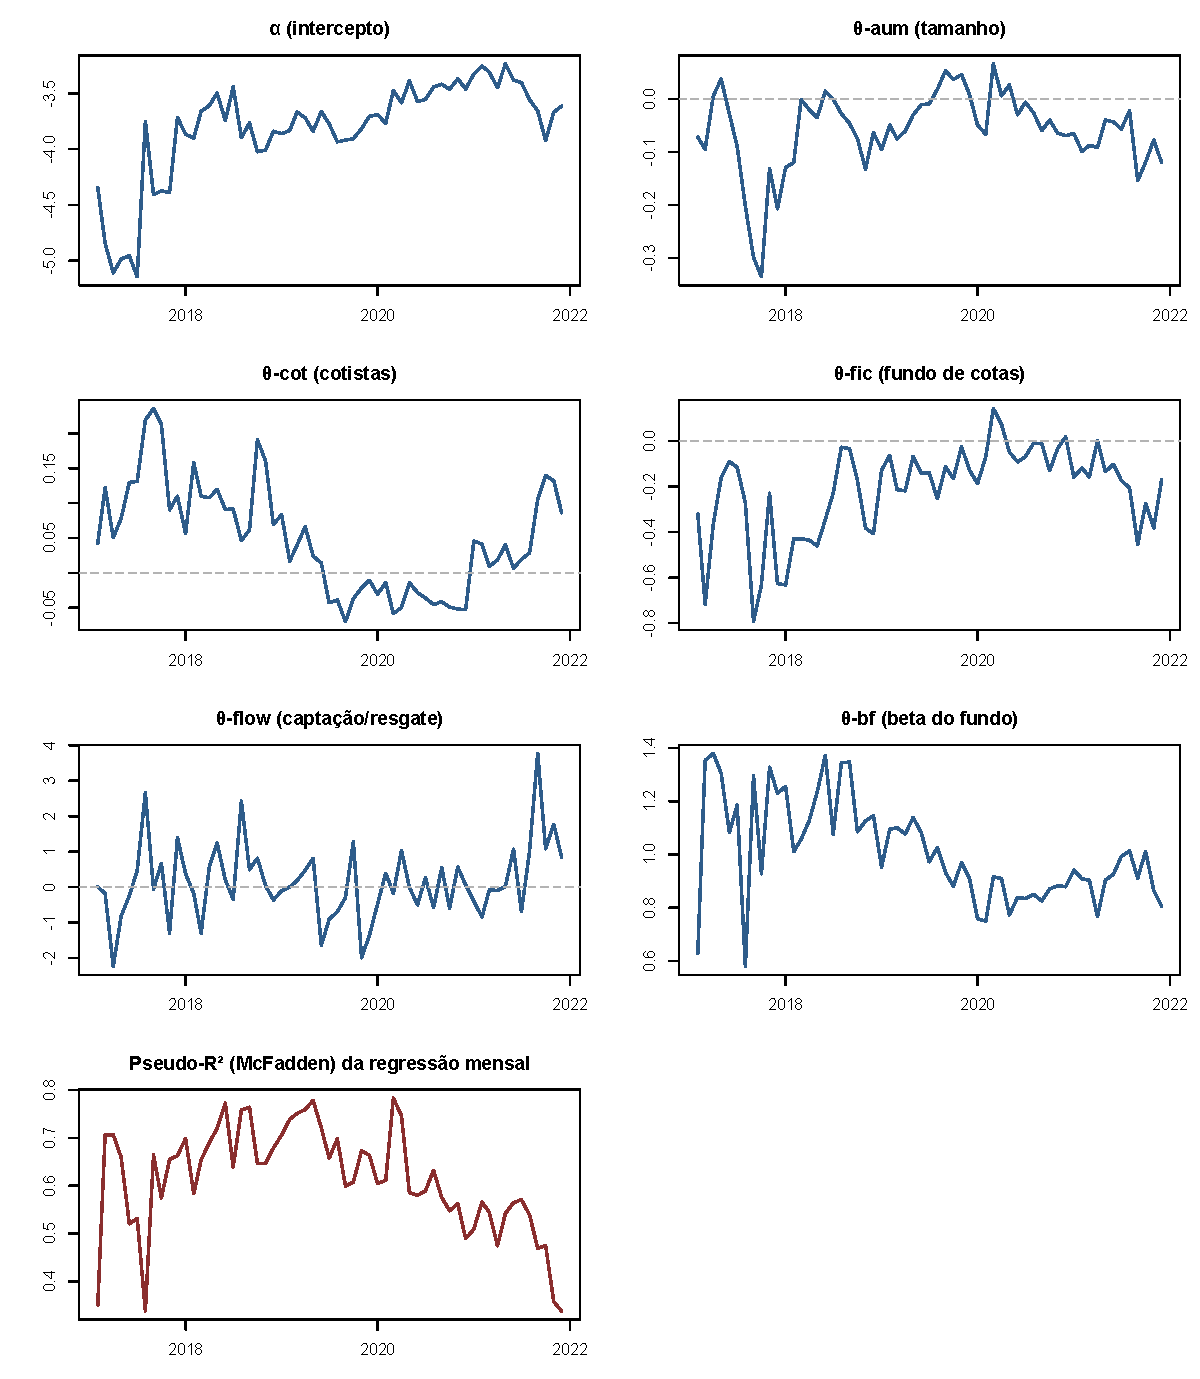
\includegraphics[width=0.75\textwidth]{fig_theta_trajetoria_v2.pdf}
\caption{Os seis componentes de $\theta_t$ logístico (com beta do fundo) ao longo dos 59 meses, e
o pseudo-$R^2$ de McFadden de cada regressão mensal. $\theta^{bf}$ é sempre positivo, coerente com
sua significância forte e estável.}
\end{figure}

\subsection{O erro $e$}

$e_{i,t}=\text{peso}_{i,t}-g(x_{i,t}'\theta_t)$, o erro de ajuste da regressão logística
(dentro da amostra).

\begin{table}[h]\centering\small
\caption{Estatísticas do erro $e$ (8.335 observações).}
\begin{tabular}{@{}lr@{}}
\toprule
Estatística & Valor \\
\midrule
Média & $0{,}000000$ \\
Desvio-padrão & $0{,}0227$ \\
Mediana & $-0{,}0008$ \\
Mínimo / Máximo & $-0{,}113$ / $0{,}178$ \\
\% de observações com $e>0$ & $45{,}1\%$ \\
Assimetria & $0{,}39$ \\
Curtose & $7{,}67$ (normal $=3$) \\
Previsões fora de $[0,1]$ & $0$ de $8.335$ \\
\bottomrule
\end{tabular}
\end{table}

A média é zero em todo mês --- mecânico (condição de primeira ordem da máxima verossimilhança
com intercepto), não evidência de bom ajuste. O desvio-padrão caiu de $0{,}0305$ (versão sem
beta do fundo) para $0{,}0227$ --- o modelo ajusta melhor, coerente com o salto no pseudo-$R^2$.

\begin{figure}[h]\centering
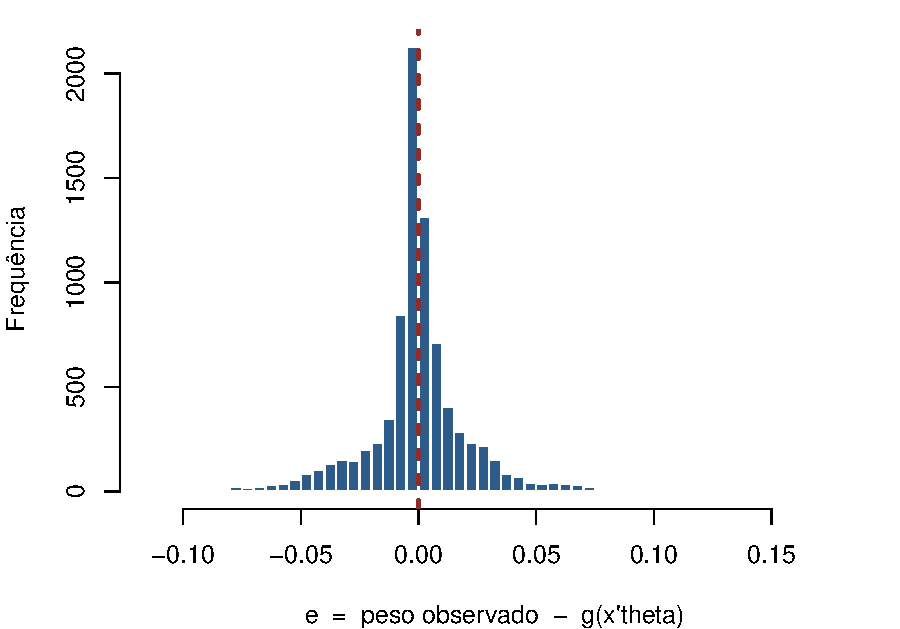
\includegraphics[width=0.7\textwidth]{hist_erro_e_v2.pdf}
\caption{Histograma do erro $e$ (8.335 observações). A linha tracejada marca zero.}
\end{figure}

\begin{figure}[h]\centering
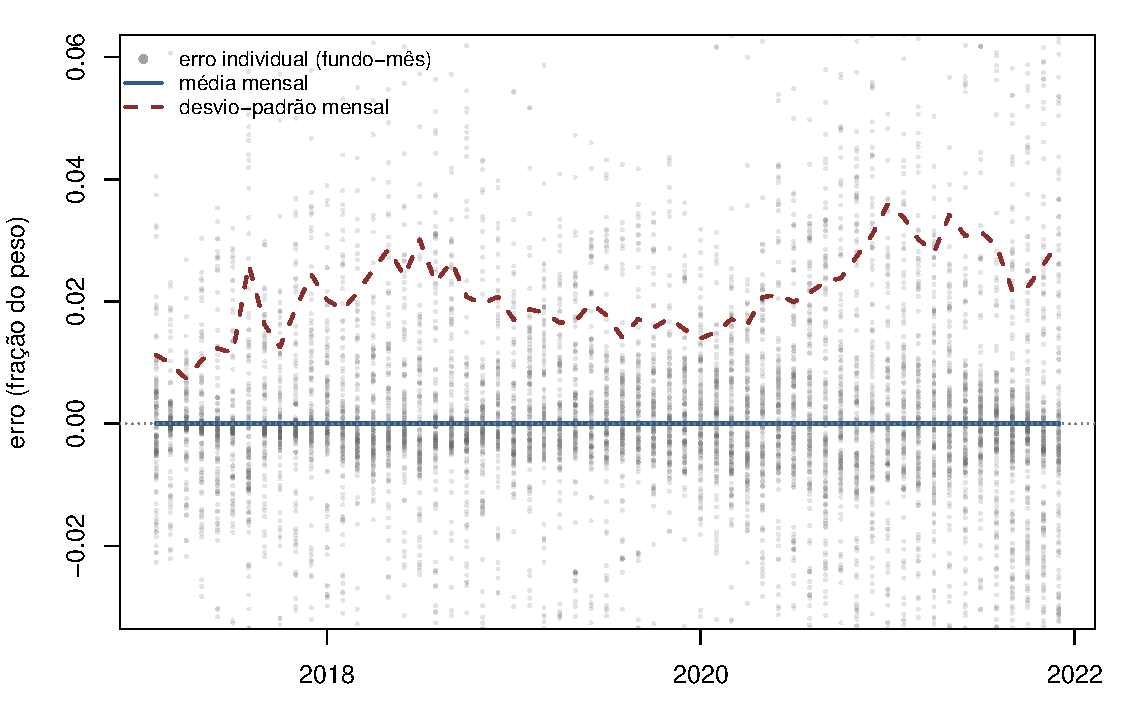
\includegraphics[width=0.78\textwidth]{fig_erro_e_mensal_v2.pdf}
\caption{Evolução mês a mês do erro $e$: nuvem cinza = erro individual de cada fundo-mês; linha
azul = média mensal (mecanicamente zero); linha vermelha tracejada = desvio-padrão mensal. Eixo
$y$ restrito a $[-0{,}03,\,0{,}06]$ para facilitar a leitura das duas linhas ---
$843$ dos $8.335$ pontos individuais ($10\%$) ficam fora e não aparecem.}
\end{figure}

% ======================================================================
\FloatBarrier
\section{Etapa 2: o ajuste parcial}

\pergunta{O peso de um fundo se move em direção ao que as características sugerem, ou fica
parado onde está?}

O alvo de um fundo, num mês, é $w^*_{i,t}=g(x_{i,t}'\theta_t)$ --- a mesma previsão da Etapa 1.
A hipótese de ajuste parcial: o fundo fecha uma fração $\lambda$ da distância ao alvo a cada mês.

\equacao
\begin{equation}
w_{i,t+1} - w_{i,t} = \lambda\, d_{i,t} + u_{i,t+1}, \qquad d_{i,t} \equiv w^*_{i,t} - w_{i,t}
\label{eq:pa}
\end{equation}
Estimado por MQO direto, sem intercepto, pooled em todos os fundo-meses --- um único método,
sem instrumento, sem efeito-fixo, sem painel dinâmico.

\subsection{O resultado}

$$\widehat\lambda = 0{,}1534 \qquad (\text{erro-padrão}=0{,}0075,\ t=20{,}6,\
R^2=0{,}050,\ n=7.987)$$

$\lambda$ subiu de $0{,}098$ (versão anterior) para $0{,}153$ --- esperado, já que o alvo $w^*$
agora é mais preciso (pseudo-$R^2$ maior na Etapa 1), o que atenua menos o coeficiente pelo erro de
medida clássico (Problema 1 do modelo de ajuste parcial). Em média, um fundo fecha $15{,}3\%$
da distância ao alvo por mês.

\subsection{O erro $u$}

\begin{table}[h]\centering\small
\caption{Estatísticas do erro $u$ (7.987 observações, pares de meses consecutivos).}
\begin{tabular}{@{}lr@{}}
\toprule
Estatística & Valor \\
\midrule
Média & $0{,}0002$ \\
Desvio-padrão & $0{,}0151$ \\
Mediana & $-0{,}0004$ \\
Mínimo / Máximo & $-0{,}160$ / $0{,}185$ \\
\% de observações com $u>0$ & $44{,}3\%$ \\
Assimetria & $0{,}59$ \\
Curtose & $19{,}4$ (normal $=3$) \\
\bottomrule
\end{tabular}
\end{table}

Praticamente idêntico ao da versão anterior (dp $0{,}0151$ nas duas) --- a mudança na Etapa 1
melhorou o ajuste de $e$, mas o comportamento do erro do ajuste parcial em si não muda muito.

\begin{figure}[h]\centering
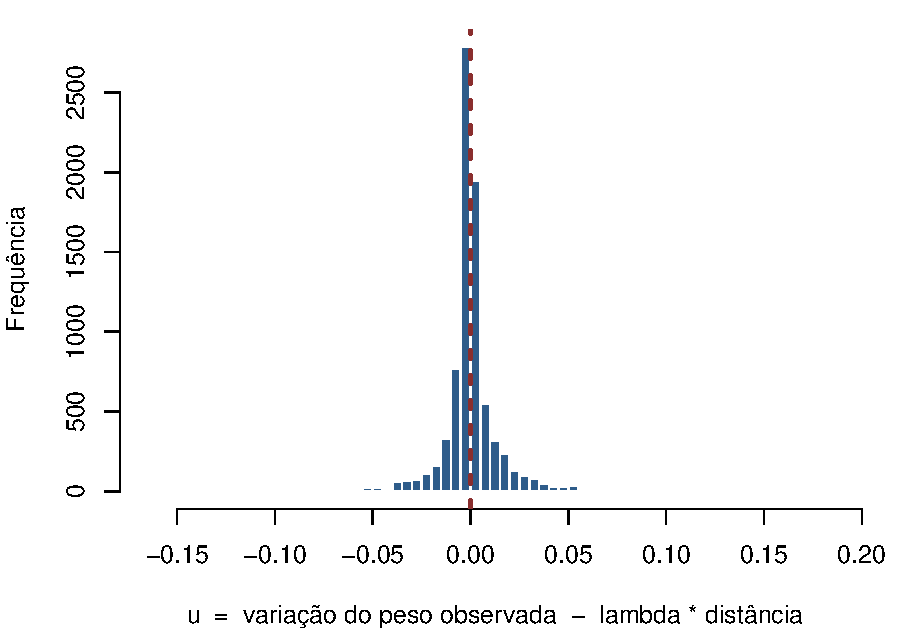
\includegraphics[width=0.7\textwidth]{hist_erro_u_v2.pdf}
\caption{Histograma do erro $u$ (7.987 observações).}
\end{figure}

\begin{figure}[h]\centering
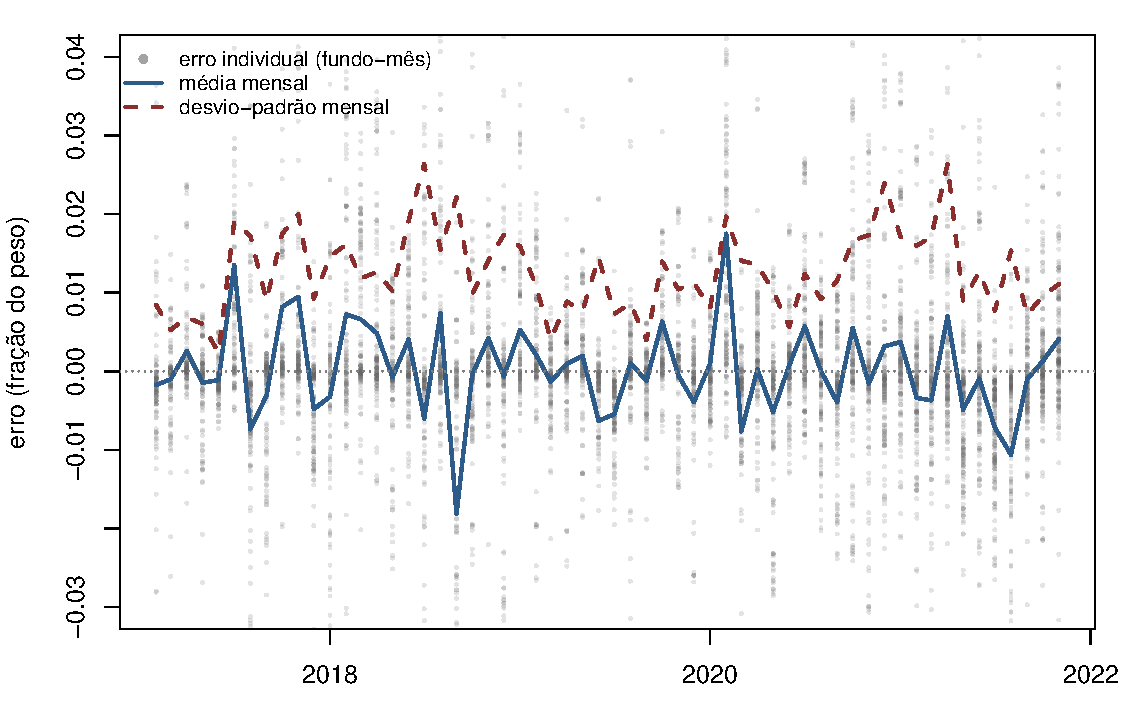
\includegraphics[width=0.78\textwidth]{fig_erro_u_mensal_v2.pdf}
\caption{Evolução mês a mês do erro $u$. Eixo $y$ restrito a $[-0{,}03,\,0{,}04]$; $369$ dos
$7.987$ pontos individuais ($4{,}6\%$) ficam fora e não aparecem.}
\end{figure}

% ======================================================================
\FloatBarrier
\section{Etapa 3: um esquema in/out-of-sample}

\pergunta{O $\lambda$ estimado serve pra prever de verdade, em dados que o modelo nunca viu?}

Um único corte no tempo, dentro do período coberto pela Etapa 1 (fev/2017 a dez/2021):

\begin{itemize}[topsep=2pt,itemsep=2pt]
\item \textbf{Treino:} 2017-02 a 2019-12 (35 meses, 4.352 observações).
\item \textbf{Teste:} 2020-01 a 2021-11 (23 meses, 3.635 observações).
\end{itemize}

\equacao
$\widehat\lambda$ é estimado pela equação~\eqref{eq:pa} só com dados de treino, depois aplicado
fixo aos meses de teste:
\begin{equation}
\widehat w_{i,t+1} = w_{i,t} + \widehat\lambda_{\text{treino}}\,d_{i,t}
\quad\text{(ajuste parcial)} \qquad\text{vs.}\qquad
\widehat w_{i,t+1} = w_{i,t} \quad\text{(ingênua)}
\label{eq:oos}
\end{equation}
$\theta_t$ continua sendo estimado mês a mês, sem vazamento de informação futura.

$$\widehat\lambda_{\text{treino}} = 0{,}1951 \qquad (\text{35 meses de treino})$$

\subsection{O resultado, fora da amostra}

\begin{table}[h]\centering\small
\caption{RMSE e MAE dentro e fora da amostra, ajuste parcial vs. ingênua.}
\begin{tabular}{@{}lrrr@{}}
\toprule
Amostra & Modelo & RMSE & MAE \\
\midrule
Treino (2017--2019) & Ajuste parcial & $0{,}01463$ & --- \\
Treino (2017--2019) & Ingênua        & $0{,}01510$ & --- \\
Teste (2020--2021)  & Ajuste parcial & $0{,}01560$ & $0{,}00906$ \\
Teste (2020--2021)  & Ingênua        & $0{,}01585$ & $0{,}00847$ \\
\bottomrule
\end{tabular}
\end{table}

\begin{figure}[h]\centering
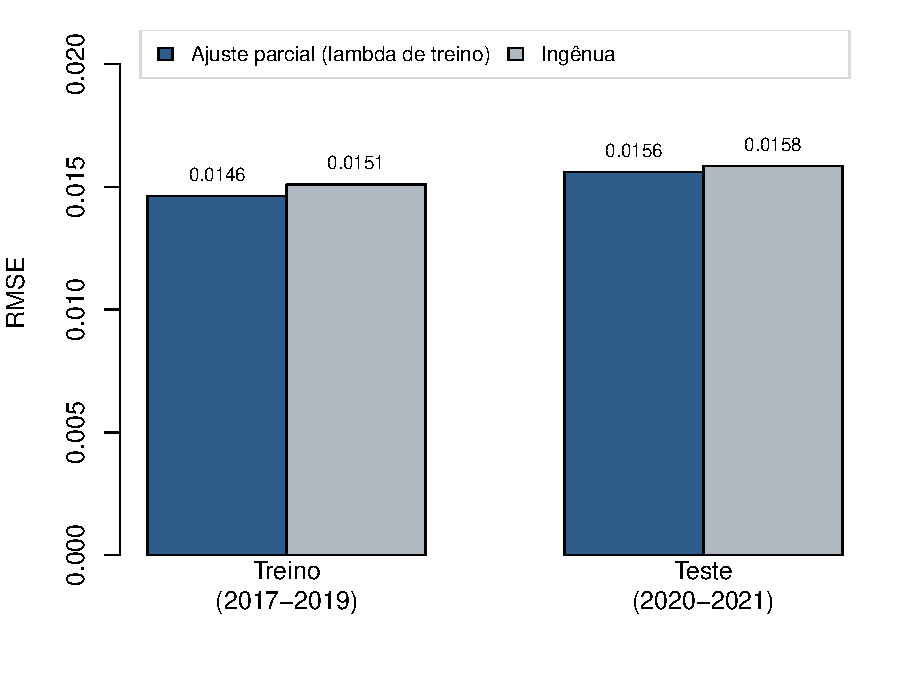
\includegraphics[width=0.68\textwidth]{fig_oos_barras_v2.pdf}
\caption{RMSE dentro (treino) e fora (teste) da amostra, ajuste parcial vs. ingênua.}
\end{figure}

O ajuste parcial vence em RMSE nas duas amostras (razão teste $=0{,}984$) --- mesmo padrão da
versão anterior. Em MAE, a ingênua continua vencendo nos casos típicos ($0{,}00847$ contra
$0{,}00906$): o ajuste parcial evita alguns erros grandes, mas erra um pouco mais em geral.
Mês a mês, vence em $14$ dos $23$ meses de teste ($61\%$).

\begin{figure}[h]\centering
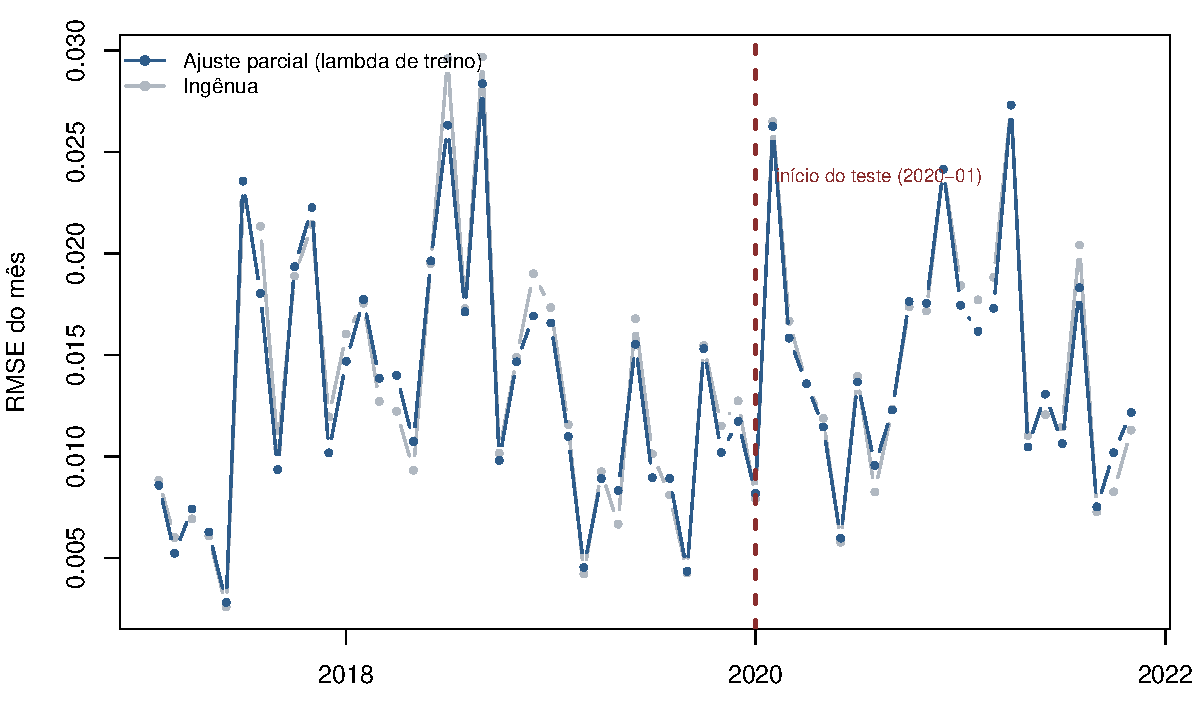
\includegraphics[width=0.85\textwidth]{fig_erro_periodo_completo_v2.pdf}
\caption{RMSE mês a mês no período completo (2017--2021). A linha vermelha tracejada marca o
início do teste (2020-01). As duas linhas seguem coladas dos dois lados do corte --- a
vantagem do ajuste parcial é pequena e consistente, não concentrada num único mês.}
\end{figure}

\subsection{RMSE flexível: o mesmo teste, em vários horizontes}

\pergunta{A vantagem do ajuste parcial sobre a ingênua (Tabela~5) é específica de prever 1 mês à
frente, ou se mantém prevendo 2, 3, 6, 12 meses à frente?}

Mesmo esquema treino/teste da Tabela~5 (treino $<$ 2020-01, teste $\geq$ 2020-01), repetido para
cada horizonte $h\in\{1,2,3,6,12\}$ meses: $dw_h=w_{i,t+h}-w_{i,t}$, $\widehat\lambda_h$ estimado
por MQO só no treino, alvo $w^*_{i,t}$ sempre fixado em $t$ (não temos características futuras
para recalculá-lo). Modelo ingênuo continua prevendo zero mudança.

\begin{table}[h]\centering\small
\caption{RMSE fora da amostra (2020--2021), ajuste parcial vs. ingênua, por horizonte.}
\begin{tabular}{@{}rrrrrrr@{}}
\toprule
$h$ (meses) & $\widehat\lambda_h$ & Meses teste & RMSE ajuste & RMSE ingênua & Margem & Vence \\
\midrule
1  & $0{,}1951$ & 23 & $0{,}01560$ & $0{,}01585$ & $1{,}5\%$ & $61\%$ \\
2  & $0{,}2502$ & 22 & $0{,}01904$ & $0{,}01957$ & $2{,}7\%$ & $59\%$ \\
3  & $0{,}2604$ & 21 & $0{,}02087$ & $0{,}02175$ & $4{,}1\%$ & $57\%$ \\
6  & $0{,}3191$ & 18 & $0{,}02472$ & $0{,}02577$ & $4{,}1\%$ & $78\%$ \\
12 & $0{,}4059$ & 12 & $0{,}02943$ & $0{,}02960$ & $0{,}6\%$ & $67\%$ \\
\bottomrule
\end{tabular}
\caption*{\footnotesize ``Margem'' = redução percentual de RMSE do ajuste parcial sobre a
ingênua; ``Vence'' = \% dos meses de teste em que o ajuste parcial tem RMSE menor naquele mês.
Fonte: elaboração própria (\texttt{scripts/36\_rmse\_multihorizonte.R}).}
\end{table}

\begin{figure}[h]\centering
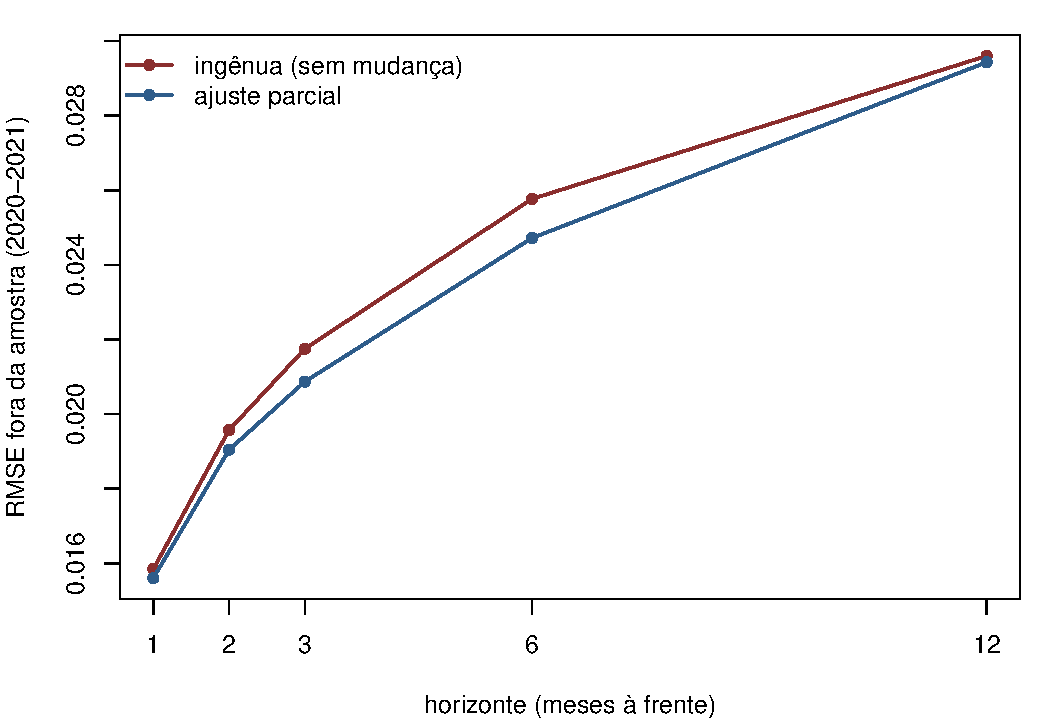
\includegraphics[width=0.75\textwidth]{fig_rmse_multihorizonte_v2.pdf}
\caption{RMSE fora da amostra, ajuste parcial vs.\ ingênua, por horizonte de previsão.}
\end{figure}

\aha{O ajuste parcial vence a ingênua em RMSE em \textbf{todos} os 5 horizontes testados --- a
vantagem não é um artefato de olhar só 1 mês à frente. Mas a margem não é estável: cresce de
$1{,}5\%$ ($h=1$) para um pico de $4{,}1\%$ ($h=3$ e $h=6$) e praticamente desaparece em $h=12$
($0{,}6\%$, com apenas $12$ meses de teste disponíveis --- amostra pequena, ler com cautela).
$\widehat\lambda_h$ cresce com o horizonte ($0{,}195\to0{,}406$), mas bem mais devagar do que uma
composição geométrica simples do $\lambda_1$ previria (12 aplicações sucessivas de
$\lambda_1=0{,}195$ fechariam $\approx93\%$ do hiato, não os $\approx41\%$ observados) --- sinal
de que o
ajuste parcial não é um processo de decaimento a taxa constante: o alvo $w^*$ também se move no
caminho, e um $\lambda$ estimado separadamente para cada horizonte capta isso melhor do que
projetar $\lambda_1$ para frente.}

% ======================================================================
\FloatBarrier
\section{Extensão: mais gestoras}
\label{sec:gestoras}

\pergunta{O padrão encontrado (tamanho, cotistas, fundo de cotas, beta do fundo explicam o
peso) é uma particularidade dos fundos do Itaú, ou aparece em qualquer gestora? E gestoras
diferentes carregam mais ou menos VALE3 do que outras, tudo o mais igual?}

Até aqui, a amostra era só os fundos do grupo Itaú. Esta extensão amplia para \textbf{todos os
fundos do universo CVM} que já tiveram VALE3 em algum momento (2016--2021) --- $2.820$ fundos,
$41$ grupos de gestora (agrupados por marca controladora; ex.: ``BTG Pactual'' junta 4 rótulos
diferentes que a CVM usa para a mesma casa). A equação~\eqref{eq:logit} ganha um efeito fixo de
gestora --- $40$ variáveis de $0$/$1$ (uma por grupo, exceto o Itaú, que fica como referência,
para não haver colinearidade perfeita com o intercepto):
$$\text{peso}_{i,t} = g\big(x_{i,t}'\theta_t + \textstyle\sum_{g\neq\text{Itaú}} \gamma_{g,t}\, D_{g,i}\big) + \text{erro}_{i,t}$$

\textbf{Adendo de processo:} ao rodar essa regressão pela primeira vez, todas as cinco
características saíram não significativas --- um resultado que parecia dizer ``a identidade da
gestora explica tudo, as características não importam mais''. Investigando, a causa não era o
efeito fixo de gestora: era \textbf{um único fundo-mês com dado corrompido} (peso de VALE3
registrado como $1.398{,}5$ --- impossível, peso é uma fração de $0$ a $1$) que, sozinho,
distorcia a regressão de um mês inteiro (set/2018). Removido esse ponto (junto com outro caso
igual, peso $=1.087{,}8$, e $13$ fundo-meses de beta do fundo com denominador degenerado por
cota irregular), o resultado abaixo é o que sobrevive.

\begin{table}[h]\centering\small
\caption{$\Theta$ logístico, amostra de todas as gestoras (59 meses, $71.569$ obs.): sem e com
efeito fixo de gestora.}
\begin{tabular}{@{}lrcrc@{}}
\toprule
Variável & Média (sem FE gestora) & Sig. & Média (com FE gestora) & Sig. \\
\midrule
$\alpha$                   & $-3{,}7989$  & *** & $-3{,}9272$  & *** \\
$\theta^{aum}$ (tamanho)        & $-0{,}0120$ & n.s. & $-0{,}0141$ & * \\
$\theta^{cot}$ (cotistas)       & $0{,}0462$  & *** & $0{,}0331$  & *** \\
$\theta^{fic}$ (fundo de cotas) & $-0{,}1641$ & *** & $-0{,}1559$ & *** \\
$\theta^{flow}$ (captação/resgate) & $-0{,}1583$ & *** & $-0{,}1254$ & *** \\
$\theta^{bf}$ (beta do fundo)   & $0{,}9052$  & *** & $0{,}8833$  & *** \\
\midrule
Pseudo-$R^2$ (McFadden) médio & $0{,}604$ & & $0{,}696$ & \\
\bottomrule
\end{tabular}
\end{table}

\begin{table}[h]\centering\small
\caption{Efeito marginal médio (APE) do logit com todas as gestoras, em pontos percentuais.}
\begin{tabular}{@{}lrcrc@{}}
\toprule
Característica & APE (sem FE gestora) & Sig. & APE (com FE gestora) & Sig. \\
\midrule
Tamanho              & $-0{,}00085$ & *** & $-0{,}00080$ & *** \\
Cotistas             & $0{,}00123$  & *** & $0{,}00079$  & *** \\
Fundo de cotas       & $-0{,}00455$ & *** & $-0{,}00424$ & *** \\
Captação/resgate     & $-0{,}00377$ & *** & $-0{,}00251$ & ** \\
Beta do fundo        & $0{,}02691$  & *** & $0{,}02635$  & *** \\
\bottomrule
\end{tabular}
\caption*{\footnotesize Fonte: elaboração própria (\texttt{scripts/20\_etapa1\_com\_gestora.R},
\texttt{23\_etapa1\_gestora\_antes\_depois.R}).}
\end{table}

\aha{Uma diferença real em relação à versão anterior (linear): no logit, \textbf{tamanho fica bem
mais fraco} --- n.s.\ sem FE, só marginal (*) com FE, contra ***/*** que a escala linear
mostrava. É o coeficiente bruto (log-odds) que perde força; o APE de tamanho continua ***
significativo nas duas colunas ($-0{,}00085$ e $-0{,}00080$), só que pequeno em magnitude --- as
duas leituras não se contradizem, só usam testes diferentes (a variação mês a mês do coeficiente
bruto é maior, em termos relativos, do que a da sua tradução em pontos percentuais). Cotistas,
FIC, fluxo e beta do fundo continuam robustamente significativos nas duas especificações. Pseudo-$R^2$
sobe de $0{,}604$ para $0{,}696$ com o efeito fixo de gestora: a identidade da gestora tem poder
explicativo próprio, mas não ``rouba'' o efeito das características --- o padrão da Etapa 1
generaliza para além do Itaú. Diferente da amostra só-Itaú (Tabela 1), aqui a captação/resgate é
claramente significativa (*** sem FE, ** com FE) --- com $71.569$ observações contra $8.335$, há
poder estatístico para detectar um efeito de fluxo pequeno que na amostra menor não era
distinguível de ruído.}

\subsection{Quanto cada gestora carrega, relativo ao Itaú}

Cada $\gamma_g$ (log-odds) é o quanto o preditor linear de um fundo da gestora $g$ se desloca em
relação a um fundo do Itaú \textbf{com as mesmas} cinco características. Como log-odds não é
diretamente interpretável, a tabela também traz o \textbf{APE discreto} de cada gestora: a
diferença média de $g(\cdot)$ forçando aquele fundo a ser da gestora $g$ contra forçá-lo a ser do
Itaú, para todos os fundos da amostra (mesma lógica do APE do FIC) --- em pontos percentuais de
peso, positivo = carrega mais VALE3 que o Itaú equivalente, negativo = carrega menos.

\textbf{Adendo de processo:} em $5$ das $40$ gestoras, o sinal do coeficiente médio (log-odds) e
do APE médio \textbf{discordam}. Não é erro: dentro de cada mês, os dois sempre têm o mesmo sinal
matematicamente (é uma propriedade de $g(\cdot)$ ser monótona) --- a discordância aparece só na
\emph{média simples ao longo dos meses}, quando o coeficiente em log-odds tem alguns meses de
magnitude extrema (comum quando a gestora tem poucos fundos naquele mês) que dominam a média bruta
mas ficam ``espremidos'' pela função logística ao virar APE. O caso mais claro é a Kinea: negativa
e com magnitude enorme em 2017--2018 (chegando a $-12{,}6$ em jun/2018), mas consistentemente
positiva e modesta de 2019 em diante --- a média do coeficiente fica negativa (dominada pelos
extremos de 2017--2018), a média do APE fica positiva (o período mais longo e mais estável de
2019--2021 pesa mais depois de passar pela função logística). Os outros $4$ casos (JGP, ARX,
Vinci Partners, Safra) têm APE tão perto de zero que o sinal é irrelevante na prática. Por isso a
tabela é ordenada pelo \textbf{APE}, a medida mais robusta a esses extremos.

\begin{center}\scriptsize
\begin{longtable}{@{}lrrcrc@{}}
\caption{Coeficiente (log-odds) e APE (pontos percentuais) de cada gestora vs.\ Itaú
(referência), ordenado pelo APE do maior para o menor.}\\
\toprule
Gestora & Meses & Coef. & Sig. & APE & Sig. \\
\midrule
\endfirsthead
\multicolumn{6}{l}{\textit{Tabela 9 (continuação)}}\\
\toprule
Gestora & Meses & Coef. & Sig. & APE & Sig. \\
\midrule
\endhead
\midrule
\multicolumn{6}{r}{\textit{continua na próxima página}}\\
\endfoot
\bottomrule
\multicolumn{6}{@{}p{0.95\textwidth}@{}}{\footnotesize ``Meses'' = quantos dos 59 meses aquela
gestora teve dados suficientes para entrar na regressão. $t$ e significância: teste ingênuo sobre
a média mensal (do coeficiente e do APE, respectivamente), mesmo estilo das demais tabelas. Fonte:
elaboração própria (\texttt{scripts/20\_etapa1\_com\_gestora.R},
\texttt{21\_coeficientes\_gestora.R}).}\\
\endlastfoot
Legacy Capital & 1 & $+2{,}3422$ & --- & $+0{,}16960$ & --- \\
Núcleo Capital & 4 & $+1{,}1618$ & *** & $+0{,}04666$ & *** \\
Occam Brasil & 59 & $+0{,}6456$ & *** & $+0{,}02703$ & *** \\
Truxt Investimentos & 42 & $+0{,}3892$ & *** & $+0{,}02071$ & *** \\
Plural & 59 & $+0{,}4350$ & *** & $+0{,}02050$ & *** \\
AZ Quest & 56 & $+0{,}2826$ & *** & $+0{,}01437$ & *** \\
Absolute Investimentos & 28 & $+0{,}1246$ & n.s. & $+0{,}01413$ & ** \\
Sharp Capital & 59 & $+0{,}2679$ & *** & $+0{,}01315$ & *** \\
Real Investor & 47 & $+0{,}2455$ & ** & $+0{,}01275$ & *** \\
SPX Capital & 59 & $+0{,}1818$ & * & $+0{,}01230$ & *** \\
Western Asset & 59 & $+0{,}3688$ & *** & $+0{,}01156$ & *** \\
Caixa & 59 & $+0{,}3634$ & *** & $+0{,}01113$ & *** \\
Dahlia Capital & 30 & $+0{,}1551$ & n.s. & $+0{,}01070$ & ** \\
Claritas Investimentos & 59 & $+0{,}2810$ & *** & $+0{,}01058$ & *** \\
Opportunity & 59 & $+0{,}1438$ & n.s. & $+0{,}01040$ & *** \\
BB Asset Management & 59 & $+0{,}3277$ & *** & $+0{,}00909$ & *** \\
Credit Suisse & 59 & $+0{,}1557$ & ** & $+0{,}00892$ & *** \\
Bradesco Asset Management & 59 & $+0{,}2945$ & *** & $+0{,}00886$ & *** \\
Santander Brasil Asset Management & 59 & $+0{,}2252$ & *** & $+0{,}00839$ & *** \\
Kinea Investimentos & 54 & $-0{,}6161$ & * & $+0{,}00555$ & * \\
BNP Paribas & 59 & $+0{,}1602$ & *** & $+0{,}00505$ & *** \\
Verde Asset Management & 59 & $+0{,}0688$ & n.s. & $+0{,}00402$ & ** \\
JGP & 59 & $-0{,}0275$ & n.s. & $+0{,}00153$ & n.s. \\
ARX Investimentos & 57 & $-0{,}4219$ & * & $+0{,}00029$ & n.s. \\
Vinci Partners & 59 & $-0{,}2411$ & ** & $+0{,}00007$ & n.s. \\
Safra Asset Management & 59 & $-0{,}0973$ & * & $+0{,}00000$ & n.s. \\
BTG Pactual & 59 & $-0{,}0914$ & * & $-0{,}00078$ & n.s. \\
Julius Baer Family Office & 59 & $-0{,}0491$ & n.s. & $-0{,}00140$ & * \\
Ibiuna Investimentos & 45 & $-0{,}5727$ & * & $-0{,}00425$ & n.s. \\
Daycoval Asset Management & 57 & $-1{,}0280$ & *** & $-0{,}00523$ & *** \\
XP & 59 & $-0{,}2856$ & *** & $-0{,}00562$ & *** \\
TNA Gestão Patrimonial & 59 & $-0{,}3059$ & *** & $-0{,}00751$ & *** \\
Squadra Investimentos & 45 & $-0{,}7695$ & * & $-0{,}00830$ & *** \\
Atmos Capital & 33 & $-0{,}4879$ & *** & $-0{,}01048$ & *** \\
Constellation Asset Management & 25 & $-1{,}9235$ & *** & $-0{,}01224$ & * \\
Gávea Investimentos & 34 & $-0{,}9917$ & *** & $-0{,}01274$ & *** \\
Bogari Capital & 11 & $-0{,}6110$ & *** & $-0{,}01484$ & *** \\
Kapitalo Investimentos & 52 & $-1{,}7679$ & *** & $-0{,}01790$ & *** \\
Forpus Capital & 33 & $-2{,}4478$ & *** & $-0{,}02059$ & *** \\
Guepardo Investimentos & 33 & $-4{,}6030$ & *** & $-0{,}02944$ & *** \\
\end{longtable}
\end{center}

\textbf{Leitura:} gestoras grandes de varejo/plataforma (Caixa, Bradesco, BB, Santander, Western
Asset) carregam \emph{mais} VALE3 que o Itaú equivalente; gestoras boutique de gestão
concentrada/high-conviction (Guepardo, Forpus, Kapitalo, Bogari, Gávea) carregam \emph{bem
menos}. Não é uma medida de causalidade --- é o resíduo estrutural, depois de controlar pelas 5
características, e a leitura mais plausível é filosofia de gestão: carteiras concentradas tendem
a evitar ``o nome que todo mundo tem'' a menos que apostem nele especificamente, diferente de uma
plataforma de varejo mais próxima de uma composição ampla.

\begin{figure}[h]\centering
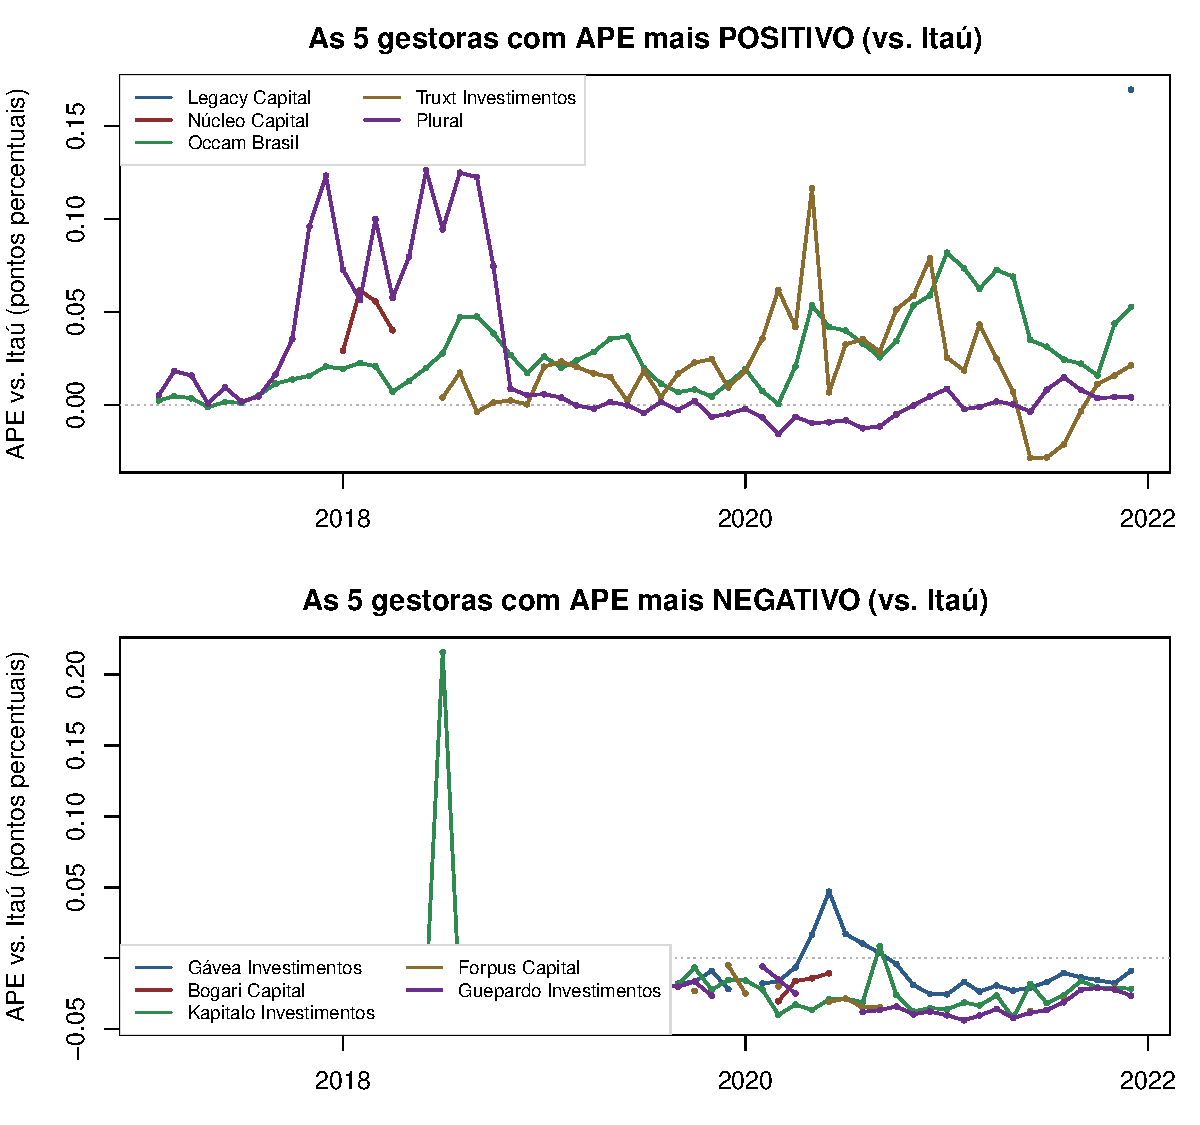
\includegraphics[width=0.85\textwidth]{fig_coef_gestora_evolucao.pdf}
\caption{Evolução mensal do APE de gestora (vs.\ Itaú, em pontos percentuais), para as 5 gestoras
com APE mais positivo e as 5 com APE mais negativo \textbf{de verdade} (mesmo ranking da
Tabela~9, sem filtro de cobertura). Duas delas têm pouquíssimos meses --- Legacy Capital ($1$ mês,
aparece como ponto isolado) e Núcleo Capital ($4$ meses) --- porque são, de fato, as gestoras com
o APE médio mais alto; não há ``evolução'' de verdade pra mostrar nesses dois casos específicos,
só o valor pontual. O pico da Kapitalo em jul/2018 não é erro de dado: naquele mês, um único
fundo da casa concentrava $37\%$ em VALE3 dentro de um grupo pequeno ($13$ fundos), o suficiente
para puxar a estimativa mensal daquele grupo --- ilustra como esses coeficientes podem ser
voláteis mês a mês quando o grupo tem poucos fundos.}
\end{figure}

% ======================================================================
\FloatBarrier
\section{Extensão: todas as ações}
\label{sec:multiativo}

\pergunta{O padrão encontrado para VALE3 é uma particularidade daquele papel, ou aparece em
qualquer ação que esses mesmos fundos carreguem?}

Mantendo o mesmo universo de $2.820$ fundos e $41$ gestoras da extensão anterior, esta seção olha
\textbf{todas as ações} que eles carregam, não só VALE3. Mesma limpeza de custódia usada no
\texttt{tcc I.pdf} (v1): a CVM registra a mesma ação sob rótulos diferentes conforme o tipo de
posição (direta, cedida/recebida em empréstimo, direito de subscrição); só a posição direta é
mantida, classificada pelo sufixo numérico do \emph{ticker} (convenção B3). Resultado: $523$
ativos de posição direta, $10.603.928$ linhas fundo-ativo-mês --- VALE3 reproduziu exatamente as
$96.349$ linhas já conhecidas, confirmando a limpeza.

\textbf{Adendo de processo:} a tabela de características (AUM/cotistas/fluxo) da Etapa 2 só
cobria os meses em que cada fundo tinha VALE3 --- $16{,}8\%$ dos fundo-mês do painel multiativo
(fundos que naquele mês só tinham \emph{outras} ações) ficavam sem essas características por um
motivo evitável, não por falta real de dado. Reconstruída usando o conjunto correto de
fundo-mês, a cobertura subiu para $97{,}6\%$. A amostra final tem $8.268.920$ linhas, $2.347$
fundos, $501$ ativos.

\textbf{Limitação conhecida:} diferente da Etapa 1/Seção~\ref{sec:gestoras} (onde o merge do beta
do fundo desloca explicitamente para o mês $t-1$), o painel multiativo desta seção em diante junta
o beta do fundo \textbf{contemporâneo} ao mês $t$, não defasado --- uma inconsistência com o
desenho ``tudo predeterminado, sem look-ahead'' descrito na Seção~\ref{sec:etapa1}. É também por
isso que este painel cobre $60$ meses (jan/2017--dez/2021) contra os $59$ da Etapa 1/Seção~5
(fev/2017 em diante): com o mês inicial contemporâneo, um mês a mais de beta fica disponível.
Testado o impacto (regressão pooled da Seção~6.2 refeita com o beta corretamente defasado):
coeficiente $0{,}867$ (era $0{,}899$), $t=30{,}2$ (era $28{,}6$), APE $0{,}00375$ (era $0{,}00462$)
--- mesma ordem de grandeza, mesmo sinal, significância igual ou mais forte. Como o beta do fundo
varia pouco de um mês para o outro (janela móvel de $252$ pregões), a defasagem de $1$ mês altera
pouco seu valor; nenhuma conclusão qualitativa das Seções~6.1--6.4 muda. Corrigido o merge e
reprocessada a seção por completo é o próximo passo natural, mas não feito nesta rodada.

\subsection{Regressão por ativo e por mês: o padrão de VALE3 generaliza?}

\equacao
\begin{align*}
\text{peso}_{i,n,t} &= g\big(x_{i,n,t}'\theta_{n,t}\big) + \text{erro} \\
x'\theta &= \alpha_{n,t} + \theta^{aum}_{n,t}z(\ln AUM_i) + \theta^{cot}_{n,t}z(\ln\text{cot}_i)
+ \theta^{fic}_{n,t}FIC_i + \theta^{flow}_{n,t}\Big(\tfrac{\text{fluxo}}{AUM}\Big)_i
+ \theta^{bf}_{n,t}z(\beta^{fundo}_i)
\end{align*}
uma regressão logística por \textbf{célula (ativo $n$, mês $t$)} com $\geq15$ fundos holders ---
mesma equação da Etapa 1 (\textbf{sem} o efeito fixo de gestora da Seção~\ref{sec:gestoras}), agora
estimada ativo a ativo. Sem gestora porque a pergunta aqui é outra: a Seção~\ref{sec:gestoras}
pergunta ``controlando por gestora, o padrão se sustenta?''; esta seção pergunta ``esse mesmo
padrão aparece em qualquer ação?'' --- para isso, já varia a regressão inteira por ativo e mês,
uma partição bem mais fina do que adicionar gestora. Na prática, também não daria: com
$15$--$20$ fundos por célula, $40$ dummies de gestora quebrariam a conta na maioria delas (mais
parâmetros que observações). $z(\cdot)$ usa a distribuição de (fundo,mês) \textbf{únicos}, não
repetida por ativo (senão um fundo com muitas posições pesaria mais na padronização). Resultado:
$13.938$ células estimadas ($19$ não convergiram, excluídas), $430$ ativos, $236$ com histórico
suficiente ($\geq24$ meses) para comparar com VALE3. Pseudo-$R^2$ médio de $0{,}441$.

\textbf{Adendo de processo:} em $12$ das $13.957$ células ($0{,}09\%$), o peso de todos os fundos
daquele ativo-mês era essencialmente zero (posição residual/legado, ex.: Cia Hering set/2021, $17$
fundos, peso $=0$ para todos) --- o denominador do pseudo-$R^2$ de McFadden colapsa nesses casos e
o valor explode para $-\infty$, não por erro de ajuste, mas por degenerescência numérica de uma
variável-resposta sem variância. Corrigido com um piso em $-1$ só nessas células (não afeta
coeficiente nem APE, só a estatística de ajuste).

A generalização é medida em dois planos, como na Seção~\ref{sec:gestoras}: pelo \textbf{sinal do
coeficiente} (log-odds) e pelo \textbf{sinal do APE} (pontos percentuais, mais robusto a
extremos).

\begin{table}[h]\centering\small
\caption{Generalização do padrão de VALE3 entre os 236 ativos com histórico suficiente.}
\begin{tabular}{@{}lrrr@{}}
\toprule
Característica & \% mesmo sinal (coef.) & \% mesmo sinal (APE) & Percentil de VALE3 (APE) \\
\midrule
Tamanho              & $55{,}9\%$ & $50{,}8\%$ (acaso) & $5{,}9$ \\
Cotistas             & $78{,}0\%$ & $73{,}3\%$ & $95{,}3$ \\
Fundo de cotas        & $55{,}9\%$ & $50{,}8\%$ (acaso) & $5{,}1$ \\
Captação/resgate     & $30{,}9\%$ (pior que o acaso) & $33{,}5\%$ (pior que o acaso) & $5{,}5$ \\
Beta do fundo        & $97{,}0\%$ & $\mathbf{96{,}2\%}$ & $99{,}6$ \\
\bottomrule
\end{tabular}
\caption*{\footnotesize Fonte: elaboração própria (\texttt{scripts/25b} a \texttt{30}).}
\end{table}

\aha{Pelo APE (a medida mais confiável), tamanho e fundo de cotas generalizam \textbf{no nível do
acaso} ($50{,}8\%$, o mesmo que uma moeda) --- mais fraco do que o sinal do coeficiente bruto já
sugeria ($55{,}9\%$), e bem mais fraco do que a v1 encontrou (tamanho/cotistas/FIC generalizando
em $88$--$98\%$ dos ativos). Captação/resgate generaliza \textbf{pior que o acaso} nos dois
planos. O beta do fundo é, disparado, o padrão mais universal: $96$--$97\%$ dos ativos têm o
mesmo sinal de VALE3, nas duas medidas. VALE3 continua extremo em quase toda dimensão do APE
(percentis abaixo de $6$ ou acima de $95$), inclusive no beta do fundo, onde fica em $2^o$ lugar
entre os $236$ ativos.}

\begin{figure}[h]\centering
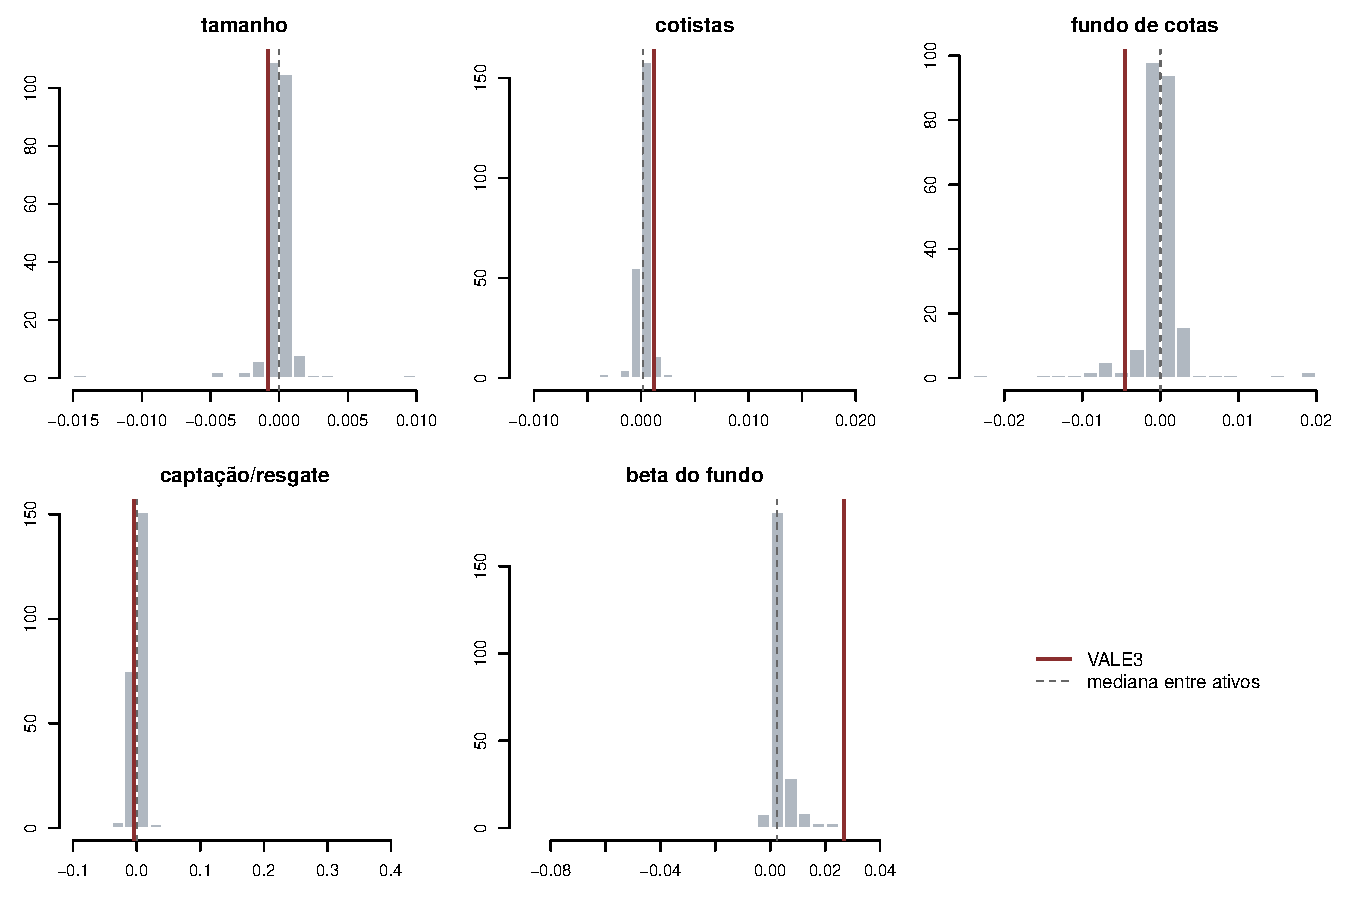
\includegraphics[width=0.92\textwidth]{fig_multiativo_dist_v2.pdf}
\caption{Distribuição do APE médio de cada característica entre os 236 ativos com histórico
suficiente (linha vermelha: VALE3; linha tracejada: mediana entre ativos).}
\end{figure}

\subsubsection*{Um panorama mais completo: além da comparação com VALE3}

A Tabela~10 sempre ancora a comparação em VALE3 --- de propósito, já que a pergunta desta seção é
se o padrão de VALE3 generaliza, não um estudo independente de demanda por todas as $236$ ações.
Mas os dados já dão pra um panorama mais amplo: a distribuição completa do APE entre os ativos, e
quem são os outros papéis nos extremos.

\begin{table}[h]\centering\small
\caption{Distribuição do APE entre os 236 ativos (quartis), com VALE3 para referência.}
\begin{tabular}{@{}lrrrr@{}}
\toprule
Característica & Q1 & Mediana & Q3 & VALE3 \\
\midrule
Tamanho          & $-0{,}00026$ & $-0{,}00000$ & $0{,}00027$ & $-0{,}00079$ \\
Cotistas         & $-0{,}00003$ & $0{,}00015$  & $0{,}00045$ & $0{,}00122$  \\
Fundo de cotas   & $-0{,}00061$ & $-0{,}00002$ & $0{,}00057$ & $-0{,}00457$ \\
Captação/resgate & $-0{,}00010$ & $0{,}00056$  & $0{,}00169$ & $-0{,}00376$ \\
Beta do fundo    & $0{,}00100$  & $0{,}00242$  & $0{,}00429$ & $0{,}02670$  \\
\bottomrule
\end{tabular}
\caption*{\footnotesize Fonte: elaboração própria (\texttt{scripts/25b} a \texttt{30}).}
\end{table}

\begin{table}[h]\centering\small
\caption{Os 5 ativos mais e menos impulsionados pelo beta do fundo (APE), entre os 236 com
histórico suficiente.}
\begin{tabular}{@{}lrr@{}}
\toprule
\multicolumn{3}{c}{\textbf{Mais impulsionados}} \\
Ativo & Meses & APE \\
\midrule
JSL ON NM - JSLG3 & 58 & $0{,}03204$ \\
VALE ON N1 - VALE3 & 60 & $0{,}02670$ \\
Petrobras PN - PETR4 & 60 & $0{,}02368$ \\
Itaú Unibanco PN N1 - ITUB4 & 60 & $0{,}02302$ \\
Bradesco PN N1 - BBDC4 & 60 & $0{,}02293$ \\
\midrule
\multicolumn{3}{c}{\textbf{Menos impulsionados (ou negativo)}} \\
Ativo & Meses & APE \\
\midrule
Alpargatas ON N1 - ALPA3 & 55 & $-0{,}00037$ \\
Magnesita SA ON NM - MAGG3 & 25 & $-0{,}00076$ \\
Terra Santa ON NM - TESA3 & 55 & $-0{,}00112$ \\
Kroton UNT N2 - KROT11 & 33 & $-0{,}00266$ \\
Klabin S/A PN N2 - KLBN4 & 39 & $-0{,}08910$ \\
\bottomrule
\end{tabular}
\caption*{\footnotesize Fonte: elaboração própria (\texttt{scripts/25b} a \texttt{30}).}
\end{table}

\textbf{Adendo de processo:} o APE da Klabin PN parece um exagero (quase $30\times$ maior em
magnitude que o segundo colocado) --- e é. Investigando célula a célula: a \textbf{mediana}
mensal do APE da Klabin é praticamente zero ($\approx-0{,}00001$), mas alguns meses (sobretudo
2020--2021) têm pseudo-$R^2$ perto de $1$ (ex.\ $0{,}998$ em abr/2021) --- sinal de célula quase
perfeitamente separada, onde o coeficiente (e o APE derivado dele) explode sem representar um
efeito econômico real. A \textbf{média} simples entre os meses fica dominada por esses poucos
casos extremos, o mesmo padrão já visto com a Kinea na Seção~\ref{sec:gestoras}. Mantido na
tabela por transparência, mas a leitura correta da Klabin é ``sem padrão claro'', não ``efeito
negativo forte''.

\aha{VALE3 é o $2^o$ mais impulsionado pelo beta do fundo entre $236$ ativos --- atrás só da
JSL Logística, uma diferença pequena ($0{,}032$ vs.\ $0{,}027$). Os outros nomes no topo (PETR4,
ITUB4, BBDC4) são, como VALE3, \emph{blue chips} muito líquidas do Ibovespa --- reforça a leitura
de que o beta do fundo captura o quão ``equity-like''/ligado ao índice é o fundo, e isso importa
mais pra decidir quanto carregar dos papéis mais representativos do mercado.}

\subsubsection*{Trazendo gestora de volta: uma regressão pooled com efeito-fixo de gestora}

\pergunta{No começo desta seção, explicamos por que a regressão por célula ativo-mês não comporta
$40$ dummies de gestora --- poucos fundos por célula, mais parâmetros que observações. Mas fica
uma pergunta em aberto: controlando por ativo e por mês, como cada gestora se compara ao Itaú
olhando a carteira de ações \textbf{inteira} dela (não só VALE3), não uma posição isolada?}

\equacao
$$\text{peso}_{i,n,g,t} = g\big(x_{i,n,t}'\theta + \alpha_n + \delta_t + \gamma_g\big)$$
uma única regressão logística com todas as $8.268.920$ observações e \textbf{três} efeitos-fixos
simultâneos --- ativo ($\alpha_n$), mês ($\delta_t$) e \textbf{gestora} ($\gamma_g$) --- em vez de
só ativo e mês, a checagem complementar sem gestora que vem a seguir, na Seção 6.2.

\textbf{Adendo de processo:} a primeira tentativa colocou gestora como \textbf{dummy} comum na
equação (as $40$ colunas, igual à Seção~\ref{sec:gestoras}) em vez de efeito-fixo --- e estourou a
memória da máquina ($16$GB, sobrando poucos MB livres, processo precisou ser encerrado
manualmente). O motivo: o \texttt{fixest} usa um algoritmo enxuto (projeções alternadas, custo
linear no número de observações) só para variáveis marcadas como efeito-fixo; uma dummy comum de
$40$ níveis, combinada com erro-padrão clusterizado em $2.347$ fundos e mais $488+60$ níveis de
efeito-fixo de ativo/mês, monta uma matriz densa grande demais. Corrigido tratando gestora como
\textbf{terceiro} efeito-fixo --- roda em $74$ segundos, memória estável.

\begin{table}[h]\centering\small
\caption{As 5 características, com efeito-fixo de ativo, mês \emph{e} gestora juntos.}
\begin{tabular}{@{}lrrcr@{}}
\toprule
Variável & Coeficiente & $t$ (cluster por fundo) & Sig. & APE \\
\midrule
Tamanho              & $-0{,}0237$ & $-1{,}13$ & n.s. & $-0{,}000121$ \\
Cotistas             & $0{,}0773$  & $4{,}72$  & *** & $0{,}000396$ \\
Fundo de cotas       & $-0{,}0499$ & $-1{,}49$ & n.s. & $-0{,}000256$ \\
Captação/resgate     & $0{,}0007$  & $0{,}56$  & n.s. & $0{,}000004$ \\
Beta do fundo        & $0{,}8486$  & $29{,}04$ & *** & $0{,}004345$ \\
\bottomrule
\end{tabular}
\caption*{\footnotesize Correlação ao quadrado $=0{,}358$. Fonte: elaboração própria
(\texttt{scripts/41\_pooled\_fe3way\_gestora\_multiativo.R}).}
\end{table}

\aha{Com efeito-fixo de gestora somado, tamanho e fundo de cotas deixam de ser sequer
marginalmente significativos (eram $t=2{,}17$ e $t=1{,}25$ na Tabela~15, sem gestora --- a
checagem da Seção 6.2, mais adiante) --- parte do que pareciam captar era, na verdade, o
\textbf{perfil típico} de cada gestora (gestoras maiores tendem a ter fundos maiores, por
exemplo), absorvido agora pela dummy de gestora. Cotistas continua *** mas cai de magnitude. O
beta do fundo \textbf{não se move} ($t=29{,}0$ vs.\ $28{,}6$) --- reforça que é o padrão mais
robusto do documento, resistente a qualquer controle adicional.}

\begin{center}\scriptsize
\begin{longtable}{@{}lrrrrr@{}}
\caption{Efeito-fixo de gestora (log-odds), centrado no Itaú, e APE (pontos percentuais) ---
painel completo de 430 ativos, não só VALE3.}\\
\toprule
Gestora & Fundos & Meses & Efeito-fixo & vs.\ Itaú & APE vs.\ Itaú \\
\midrule
\endfirsthead
\multicolumn{6}{l}{\textit{Tabela 14 (continuação)}}\\
\toprule
Gestora & Fundos & Meses & Efeito-fixo & vs.\ Itaú & APE vs.\ Itaú \\
\midrule
\endhead
\midrule
\multicolumn{6}{r}{\textit{continua na próxima página}}\\
\endfoot
\bottomrule
\multicolumn{6}{@{}p{0.95\textwidth}@{}}{\footnotesize APE = diferença média de peso previsto
(pontos percentuais), forçando cada fundo-mês da amostra a ser da gestora indicada em vez do
Itaú, mantendo ativo, mês e as 5 características observadas -- mesma lógica do APE discreto da
Tabela~9, adaptada pra efeito-fixo em vez de dummy. Fonte: elaboração própria
(\texttt{scripts/41\_pooled\_fe3way\_gestora\_multiativo.R}).}\\
\endlastfoot
Guepardo Investimentos & 15 & 60 & $1{,}897$ & $+2{,}185$ & $+0{,}02450$ \\
Núcleo Capital & 19 & 60 & $1{,}567$ & $+1{,}855$ & $+0{,}01720$ \\
Bogari Capital & 16 & 60 & $1{,}189$ & $+1{,}477$ & $+0{,}01103$ \\
Real Investor & 5 & 60 & $1{,}151$ & $+1{,}439$ & $+0{,}01052$ \\
Ibiuna Investimentos & 8 & 60 & $1{,}046$ & $+1{,}335$ & $+0{,}00920$ \\
Legacy Capital & 1 & 2 & $1{,}038$ & $+1{,}327$ & $+0{,}00910$ \\
Constellation Asset Management & 28 & 60 & $0{,}936$ & $+1{,}225$ & $+0{,}00793$ \\
Sharp Capital & 35 & 60 & $0{,}883$ & $+1{,}171$ & $+0{,}00736$ \\
Claritas Investimentos & 15 & 60 & $0{,}821$ & $+1{,}109$ & $+0{,}00674$ \\
Squadra Investimentos & 20 & 60 & $0{,}812$ & $+1{,}101$ & $+0{,}00666$ \\
Atmos Capital & 32 & 60 & $0{,}807$ & $+1{,}096$ & $+0{,}00661$ \\
Forpus Capital & 3 & 60 & $0{,}787$ & $+1{,}076$ & $+0{,}00642$ \\
Plural & 15 & 60 & $0{,}734$ & $+1{,}022$ & $+0{,}00592$ \\
Gávea Investimentos & 17 & 60 & $0{,}724$ & $+1{,}012$ & $+0{,}00583$ \\
Kinea Investimentos & 10 & 60 & $0{,}719$ & $+1{,}008$ & $+0{,}00579$ \\
Truxt Investimentos & 31 & 43 & $0{,}681$ & $+0{,}969$ & $+0{,}00545$ \\
AZ Quest & 24 & 60 & $0{,}656$ & $+0{,}945$ & $+0{,}00524$ \\
Verde Asset Management & 15 & 60 & $0{,}561$ & $+0{,}849$ & $+0{,}00448$ \\
Absolute Investimentos & 7 & 29 & $0{,}559$ & $+0{,}848$ & $+0{,}00447$ \\
ARX Investimentos & 15 & 60 & $0{,}553$ & $+0{,}842$ & $+0{,}00442$ \\
JGP & 46 & 60 & $0{,}470$ & $+0{,}759$ & $+0{,}00381$ \\
Vinci Partners & 55 & 60 & $0{,}462$ & $+0{,}750$ & $+0{,}00375$ \\
Occam Brasil & 29 & 60 & $0{,}425$ & $+0{,}714$ & $+0{,}00350$ \\
Opportunity & 25 & 60 & $0{,}405$ & $+0{,}694$ & $+0{,}00336$ \\
Credit Suisse & 76 & 60 & $0{,}351$ & $+0{,}639$ & $+0{,}00301$ \\
SPX Capital & 37 & 60 & $0{,}284$ & $+0{,}572$ & $+0{,}00261$ \\
Dahlia Capital & 18 & 31 & $0{,}282$ & $+0{,}571$ & $+0{,}00259$ \\
BTG Pactual & 157 & 60 & $0{,}278$ & $+0{,}567$ & $+0{,}00257$ \\
Western Asset & 31 & 60 & $0{,}232$ & $+0{,}521$ & $+0{,}00231$ \\
Safra Asset Management & 156 & 60 & $0{,}216$ & $+0{,}505$ & $+0{,}00222$ \\
Kapitalo Investimentos & 22 & 60 & $0{,}158$ & $+0{,}447$ & $+0{,}00190$ \\
BB Asset Management & 116 & 60 & $0{,}112$ & $+0{,}400$ & $+0{,}00167$ \\
Caixa & 29 & 60 & $0{,}098$ & $+0{,}387$ & $+0{,}00160$ \\
Santander Brasil Asset Management & 98 & 60 & $0{,}039$ & $+0{,}328$ & $+0{,}00132$ \\
Bradesco Asset Management & 331 & 60 & $0{,}000$ & $+0{,}289$ & $+0{,}00113$ \\
BNP Paribas & 58 & 60 & $-0{,}018$ & $+0{,}271$ & $+0{,}00106$ \\
Julius Baer Family Office & 65 & 60 & $-0{,}033$ & $+0{,}256$ & $+0{,}00099$ \\
TNA Gestão Patrimonial & 33 & 60 & $-0{,}098$ & $+0{,}190$ & $+0{,}00071$ \\
XP & 104 & 60 & $-0{,}227$ & $+0{,}062$ & $+0{,}00022$ \\
Daycoval Asset Management & 6 & 60 & $-0{,}288$ & $+0{,}001$ & $+0{,}00000$ \\
Itaú & 524 & 60 & $-0{,}289$ & $0{,}000$ & $0{,}00000$ \\
\end{longtable}
\end{center}

\textbf{Adendo de processo:} diferente do resto do documento (Tabelas~9 e 18 sempre mostram
cobertura ao lado do ranking por gestora), esta tabela precisou de uma coluna nova de
\textbf{fundos}: sem ela, o ranking esconde que os extremos tendem a ser gestoras com \textbf{poucos}
fundos --- correlação de $-0{,}47$ entre nº de fundos e $|\text{efeito-fixo vs.\ Itaú}|$ ($-0{,}56$
com o log; $-0{,}35$ na escala do APE). É o padrão estatístico esperado (menos fundos = mais ruído na
estimativa do efeito-fixo daquela gestora), não um erro de cálculo --- mas fica mais claro com a
coluna à vista: a \textbf{Legacy Capital} ($6^o$ lugar) tem só $1$ fundo em $2$ meses; Real Investor
($4^o$) e Forpus ($12^o$) têm $5$ e $3$ fundos. Mesmo a \textbf{Guepardo}, no topo, tem só $15$
fundos --- poucos perto do Itaú ($524$) ou Bradesco ($331$), que ficam nos dois últimos lugares. Não
invalida o achado (fica reforçado pela Tabela~18, uma metodologia bem diferente), mas os extremos com
cobertura baixa devem ser lidos como \textbf{estimativas menos precisas}, não necessariamente como
os desvios econômicos mais extremos de verdade.

\aha{A ordem quase se \textbf{inverte} em relação à Seção~\ref{sec:gestoras}: lá (só VALE3),
gestoras de varejo/plataforma (Caixa, BB, Santander, Western Asset) carregavam \textbf{mais} VALE3
que o Itaú, e boutiques concentradas (Guepardo, Forpus, Constellation, Bogari, Atmos, Squadra)
carregavam \textbf{menos}. Aqui, olhando a carteira de ações inteira (não só VALE3), são
justamente as boutiques que têm o efeito-fixo mais alto --- Guepardo, Núcleo Capital e Bogari no
topo --- e o Itaú fica \textbf{na última posição}, junto de Daycoval. Em pontos percentuais (APE):
um fundo com o perfil da \textbf{Guepardo} carrega, em média, $2{,}45$ pontos percentuais a mais
naquele ativo do que um fundo equivalente do Itaú; Núcleo Capital, $1{,}72$ pp; Bogari, $1{,}10$ pp
--- efeitos grandes perto da mediana da amostra. Não é uma contradição com a Seção~5: as
duas coisas podem ser verdade ao mesmo tempo --- gestoras de convicção concentrada tendem a montar
posições \textbf{maiores} em geral (é o estilo delas), mas em VALE3 especificamente, um blue chip
mega-cap do Ibovespa, preferem ficar \textbf{abaixo} do Itaú (evitam ``o nome que todo mundo
tem''). Essa leitura também bate com a Seção~\ref{sec:erro-multiativo} (Tabela~18): a mesma
Guepardo e a mesma Núcleo Capital têm o viés mais positivo do erro por gestora --- duas
metodologias bem diferentes (coeficiente estrutural vs.\ resíduo agregado) chegando à mesma
ordenação, o que reforça que o padrão é real, não um artefato de uma escolha de modelo específica.}

\subsection{Checagem complementar: uma única regressão com efeito-fixo de ativo e de mês}

Como checagem independente, uma regressão logística \emph{pooled} com todas as $8.268.920$
observações, efeito-fixo de ativo \emph{e} de mês, erro-padrão agrupado por fundo --- o
coeficiente ``dentro'' de cada ativo-mês, líquido de qualquer nível particular daquele ativo ou
choque daquele mês. O truque de demeaning (Frisch--Waugh--Lovell) usado na versão linear
\textbf{não} funciona em modelos não-lineares; esta versão usa o pacote \texttt{fixest}
(\texttt{feglm}), feito especificamente para efeito-fixo em GLM de forma rápida mesmo com muitos
níveis --- aqui, $501$ ativos $+$ $60$ meses.

\textbf{Adendo de processo:} $13$ efeitos-fixos de ativo ($49$ observações) foram removidos
automaticamente por terem só um desfecho (\emph{singleton}) --- rotina do próprio
\texttt{fixest}, não afeta o resultado. Diferente da versão linear (onde o fundo de cotas saía
\textbf{exatamente} da equação, absorvido por completo pelos efeitos-fixos), aqui o FIC
\textbf{sobrevive} --- o logit não sofre da mesma colinearidade exata que a demeaning linear
sofria, porque a estimação não depende de inverter a mesma matriz.

\begin{table}[h]\centering\small
\caption{Regressão logística pooled com efeito-fixo de ativo e de mês (8.268.871 obs., 488
ativos, 60 meses, 2.347 fundos).}
\begin{tabular}{@{}lrrcr@{}}
\toprule
Variável & Coeficiente & $t$ (cluster por fundo) & Sig. & APE \\
\midrule
Tamanho              & $0{,}0490$  & $2{,}17$  & *   & $0{,}000252$ \\
Cotistas             & $0{,}0094$  & $0{,}50$  & n.s. & $0{,}000048$ \\
Fundo de cotas       & $0{,}0497$  & $1{,}25$  & n.s. & $0{,}000255$ \\
Captação/resgate     & $-0{,}0010$ & $-0{,}82$ & n.s. & $-0{,}000005$ \\
Beta do fundo        & $0{,}8994$  & $28{,}60$ & *** & $0{,}004619$ \\
\bottomrule
\end{tabular}
\caption*{\footnotesize Correlação ao quadrado $=0{,}314$ (estatística reportada pelo
\texttt{fixest}, não é o pseudo-$R^2$ de McFadden usado nas demais tabelas). Fonte: elaboração
própria (\texttt{scripts/31\_pooled\_fe2way\_multiativo.R}).}
\end{table}

\aha{As duas abordagens --- regressão por ativo-mês e pooled com efeito-fixo --- convergem para
a mesma conclusão: o beta do fundo é, disparado, a característica que mais robustamente explica
o peso de \textbf{qualquer} ação carregada por esses fundos ($t=28{,}6$, APE $\approx18\times$
maior que o de qualquer outra característica). Tamanho fica só marginalmente significativo
($t=2{,}17$); cotistas, FIC e fluxo não são distinguíveis de zero nesta especificação --- mesmo
padrão qualitativo da checagem por ativo-mês (Seção 6.1): o que na v1 parecia um efeito robusto
de tamanho/cotistas/FIC, testado no universo amplo de gestoras e ações com o beta do fundo como
controle, perde quase toda a força. Boa parte do que pareciam explicar era, plausivelmente, um
proxy indireto para o quão ``equity-like'' o fundo é.}

\subsubsection*{Um panorama mais completo: o efeito-fixo de cada ativo}

A Tabela~15 resume só os $5$ coeficientes pooled --- comuns a todos os ativos. Mas o modelo com
efeito-fixo de ativo estima, como subproduto, um nível \textbf{próprio para cada um dos $488$
ativos} (o quanto aquele papel é sobre- ou sub-pesado, líquido das $5$ características e do mês).
Vale a pena olhar essa distribuição.

\textbf{Adendo de processo:} extrair o efeito-fixo bruto direto (\texttt{fixef(f)\$ativo}) reproduz
o mesmo problema já visto na Tabela~12 (Klabin): os extremos ficam dominados por ativos com peso
\textbf{mediano} praticamente zero --- posições residuais presentes em muitos meses mas nunca
efetivamente alocadas, cujo efeito-fixo é instável sem representar demanda real (ex.: papéis com
peso mediano da ordem de $10^{-7}$ a $10^{-9}$, mesmo com $60$ meses de ``cobertura''). O filtro de
$\geq24$ meses (usado em toda a Seção~6) não resolve isso --- meses de presença não é o mesmo que
peso relevante. A tabela abaixo usa por isso um filtro adicional: peso mediano $>0{,}1\%$, o que
deixa $60$ dos $488$ ativos.

\begin{table}[h]\centering\small
\caption{Distribuição do efeito-fixo de ativo (log-odds, escala do modelo pooled) entre os 60
ativos com posição relevante ($\geq24$ meses e peso mediano $>0{,}1\%$).}
\begin{tabular}{@{}lrrr@{}}
\toprule
Q1 & Mediana & Q3 & VALE3 \\
\midrule
$-5{,}123$ & $-4{,}784$ & $-4{,}315$ & $-3{,}407$ \\
\bottomrule
\end{tabular}
\caption*{\footnotesize Fonte: elaboração própria (\texttt{scripts/39\_panorama\_fe\_ativo.R}).}
\end{table}

\begin{table}[h]\centering\small
\caption{Os 5 ativos com efeito-fixo mais alto e mais baixo, entre os 60 com posição relevante.}
\begin{tabular}{@{}lrrr@{}}
\toprule
\multicolumn{4}{c}{\textbf{Efeito-fixo mais alto (sobrepeso)}} \\
Ativo & Efeito-fixo & Meses & Peso mediano \\
\midrule
Döhler PN - DOHL4 & $-1{,}698$ & 60 & $21{,}02\%$ \\
Coelba ON - CEEB3 & $-1{,}957$ & 60 & $5{,}63\%$ \\
Celpe ON - CEPE3 & $-2{,}406$ & 60 & $1{,}63\%$ \\
Cosern ON - CSRN3 & $-2{,}837$ & 60 & $1{,}82\%$ \\
VALE ON N1 - VALE3 & $-3{,}407$ & 60 & $1{,}57\%$ \\
\midrule
\multicolumn{4}{c}{\textbf{Efeito-fixo mais baixo (subpeso)}} \\
Ativo & Efeito-fixo & Meses & Peso mediano \\
\midrule
Gerdau Met PN N1 - GOAU4 & $-5{,}488$ & 60 & $0{,}12\%$ \\
Eletrobras ON N1 - ELET3 & $-5{,}492$ & 60 & $0{,}12\%$ \\
Eletrobras PNB N1 - ELET6 & $-5{,}569$ & 60 & $0{,}13\%$ \\
WLM Ind Com PN - WLMM4 & $-6{,}079$ & 52 & $0{,}13\%$ \\
D H B PN - DHBI4 & $-6{,}586$ & 45 & $0{,}22\%$ \\
\bottomrule
\end{tabular}
\caption*{\footnotesize Fonte: elaboração própria (\texttt{scripts/39\_panorama\_fe\_ativo.R}).}
\end{table}

\aha{VALE3 fica em $5^o$ lugar entre $60$ ativos com posição relevante --- no quarto superior da
distribuição, mas não isolada: Döhler, Coelba, Celpe e Cosern têm efeito-fixo ainda mais alto.
Nenhum nome no topo ou na base é posição residual (todos com peso mediano acima de $0{,}1\%$,
alguns como a Döhler acima de $20\%$) --- ao contrário da tentativa sem filtro, aqui os extremos
refletem sobre-/sub-peso genuíno, não ruído de posições nunca alocadas.}

\subsection{O erro por gestora, agora com todas as ações}
\label{sec:erro-multiativo}

\pergunta{A regressão da Seção~\ref{sec:multiativo} cobre agora os 501 ativos, não só VALE3.
Como se comporta o erro dela quando agregado por gestora --- olhando a carteira inteira de ações,
não só uma posição?}

\equacao
$$\text{erro}_{i,n,t} = \text{peso}_{i,n,t} - g\big(x_{i,n,t}'\theta_{n,t}\big)$$
o resíduo (escala da resposta) da mesma regressão logística por célula (ativo $n$, mês $t$) da
Seção~\ref{sec:multiativo} --- $8.251.936$ observações, $430$ ativos, $2.347$ fundos, $41$
gestoras.

\textbf{Adendo de processo:} diferente de uma especificação com efeito-fixo de gestora (equação
da Seção~\ref{sec:gestoras}, onde as equações normais do MQO garantem soma-zero do resíduo dentro
de cada grupo com dummy própria), aqui \textbf{cada célula tem sua própria regressão, sem dummy
de gestora}. A
média do erro por gestora, portanto, \textbf{não} é zero por construção --- é genuinamente
informativa, junto com a dispersão. Um \textbf{viés} positivo aqui não é sobre um papel só: como
a regressão roda célula a célula (um ativo por vez) e depois o erro de cada célula é agregado por
gestora, um viés positivo significa que, \textbf{olhando o book de ações inteiro daquela
gestora}, os fundos dela carregam sistematicamente mais peso do que as 5 características previam
--- um padrão que se repete ação após ação, não um desvio pontual. Viés negativo é o oposto:
carregam menos do que a fórmula prevê, de forma consistente. Significância da média testada pela
série \textbf{mensal} por gestora (mesmo estilo do resto do documento:
$t=\bar e/(\text{dp}(e)/\sqrt{\text{meses}})$), não pelas $8,25$ milhões de observações brutas
(que tornaria qualquer diferença minúscula
``significativa'' só pelo tamanho da amostra).

\begin{center}\scriptsize
\begin{longtable}{@{}lrrrc r@{}}
\caption{Erro médio (testado pela série mensal) e dispersão, por gestora, no universo de todas
as ações --- ordenado do viés mais positivo ao mais negativo.}\\
\toprule
Gestora & Obs. & Meses & Média & Sig. & dp \\
\midrule
\endfirsthead
\multicolumn{6}{l}{\textit{Tabela 18 (continuação)}}\\
\toprule
Gestora & Obs. & Meses & Média & Sig. & dp \\
\midrule
\endhead
\midrule
\multicolumn{6}{r}{\textit{continua na próxima página}}\\
\endfoot
\bottomrule
\multicolumn{6}{@{}p{0.95\textwidth}@{}}{\footnotesize Fonte: elaboração própria
(\texttt{scripts/37\_erro\_multiativo.R}, \texttt{38\_erro\_multiativo\_gestora.R}).}\\
\endlastfoot
Guepardo Investimentos & 10798 & 60 & $+0{,}04493$ & *** & $0{,}06789$ \\
Núcleo Capital & 12247 & 60 & $+0{,}03780$ & *** & $0{,}02874$ \\
Ibiuna Investimentos & 11381 & 60 & $+0{,}01854$ & *** & $0{,}02387$ \\
Constellation Asset Management & 17423 & 60 & $+0{,}01471$ & *** & $0{,}02475$ \\
Bogari Capital & 21809 & 60 & $+0{,}01369$ & *** & $0{,}01779$ \\
Real Investor & 8244 & 60 & $+0{,}01326$ & *** & $0{,}02169$ \\
Squadra Investimentos & 20929 & 60 & $+0{,}01023$ & *** & $0{,}02823$ \\
Sharp Capital & 37399 & 60 & $+0{,}00975$ & *** & $0{,}02503$ \\
Atmos Capital & 52386 & 60 & $+0{,}00948$ & *** & $0{,}02036$ \\
Kinea Investimentos & 10045 & 60 & $+0{,}00719$ & *** & $0{,}02156$ \\
Verde Asset Management & 26440 & 60 & $+0{,}00662$ & *** & $0{,}02089$ \\
Forpus Capital & 10275 & 60 & $+0{,}00556$ & *** & $0{,}01817$ \\
Legacy Capital & 203 & 2 & $+0{,}00537$ & *** & $0{,}01769$ \\
Truxt Investimentos & 54176 & 43 & $+0{,}00537$ & *** & $0{,}01582$ \\
AZ Quest & 49444 & 60 & $+0{,}00499$ & *** & $0{,}01590$ \\
ARX Investimentos & 21290 & 60 & $+0{,}00495$ & *** & $0{,}01740$ \\
Claritas Investimentos & 24505 & 60 & $+0{,}00471$ & *** & $0{,}01405$ \\
JGP & 109991 & 60 & $+0{,}00243$ & *** & $0{,}01165$ \\
Absolute Investimentos & 20370 & 29 & $+0{,}00222$ & *** & $0{,}01190$ \\
Vinci Partners & 139937 & 60 & $+0{,}00208$ & *** & $0{,}01676$ \\
Opportunity & 54794 & 60 & $+0{,}00172$ & *** & $0{,}01728$ \\
Occam Brasil & 75151 & 60 & $+0{,}00171$ & *** & $0{,}01075$ \\
Gávea Investimentos & 13274 & 60 & $+0{,}00117$ & *** & $0{,}00434$ \\
Western Asset & 77814 & 60 & $+0{,}00110$ & *** & $0{,}01450$ \\
Plural & 17821 & 60 & $+0{,}00094$ & ** & $0{,}01099$ \\
Dahlia Capital & 36938 & 31 & $+0{,}00075$ & *** & $0{,}00620$ \\
Credit Suisse & 250452 & 60 & $+0{,}00069$ & *** & $0{,}00925$ \\
BTG Pactual & 519772 & 60 & $+0{,}00068$ & *** & $0{,}01388$ \\
SPX Capital & 126811 & 60 & $+0{,}00052$ & * & $0{,}01068$ \\
Kapitalo Investimentos & 94846 & 60 & $+0{,}00029$ & * & $0{,}00945$ \\
Safra Asset Management & 561779 & 60 & $+0{,}00022$ & *** & $0{,}00871$ \\
Caixa & 70924 & 60 & $+0{,}00006$ & n.s. & $0{,}01491$ \\
BB Asset Management & 338730 & 60 & $-0{,}00007$ & n.s. & $0{,}01485$ \\
Santander Brasil Asset Management & 348279 & 60 & $-0{,}00036$ & *** & $0{,}00841$ \\
Julius Baer Family Office & 273717 & 60 & $-0{,}00039$ & *** & $0{,}00736$ \\
TNA Gestão Patrimonial & 262921 & 60 & $-0{,}00040$ & *** & $0{,}00507$ \\
BNP Paribas & 247947 & 60 & $-0{,}00059$ & *** & $0{,}01089$ \\
XP & 391636 & 60 & $-0{,}00065$ & *** & $0{,}01141$ \\
Bradesco Asset Management & 930672 & 60 & $-0{,}00095$ & *** & $0{,}01095$ \\
Itaú & 2882582 & 60 & $-0{,}00120$ & *** & $0{,}00649$ \\
Daycoval Asset Management & 15784 & 60 & $-0{,}00211$ & *** & $0{,}00944$ \\
\end{longtable}
\end{center}

\begin{figure}[h]\centering
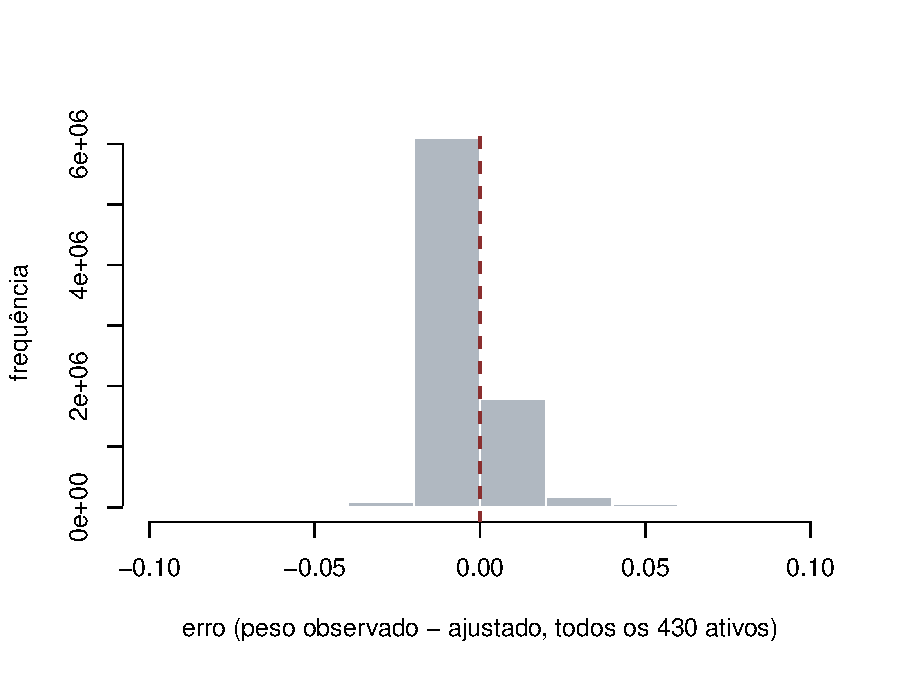
\includegraphics[width=0.75\textwidth]{hist_erro_multiativo_v2.pdf}
\caption{Distribuição do erro no universo multiativo, $8.251.936$ observações.}
\end{figure}

\aha{$36$ das $41$ gestoras têm viés estatisticamente significativo a $0{,}1\%$ (mais $1$ a $1\%$,
$2$ a $5\%$, e só $2$ n.s.\@: Caixa, BB Asset Management) --- mas a maioria das magnitudes é
pequena; a significância generalizada reflete o tamanho da amostra ($8,25$ milhões de obs.), não
necessariamente relevância econômica. A \textbf{Guepardo} tem o viés mais positivo
($+0{,}045$), seguida de perto pela Núcleo Capital ($+0{,}038$) --- olhando a carteira de ações
inteira, não só VALE3, as duas sobre-pesam sistematicamente o que a fórmula prevê, e a Guepardo
também tem, disparada, a maior dispersão ($0{,}068$, mais que o dobro da segunda colocada). O
Itaú fica com viés pequeno e negativo ($-0{,}0012$) e dispersão baixa ($0{,}0065$, abaixo da
mediana de $0{,}0145$) --- relativamente ``previsível'' nesse universo amplo.}

\begin{figure}[h]\centering
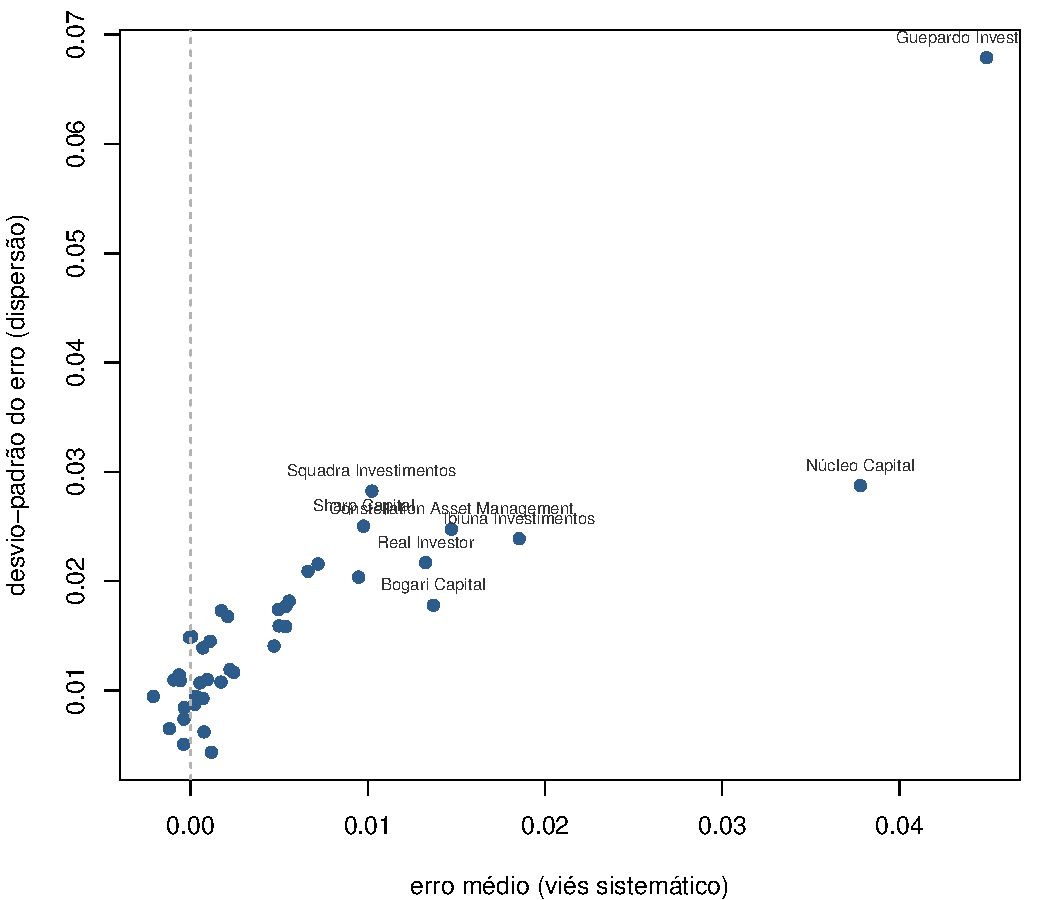
\includegraphics[width=0.85\textwidth]{fig_erro_multiativo_media_dp.pdf}
\caption{Cada ponto é uma gestora: erro médio (eixo $x$) vs.\ dispersão do erro (eixo $y$).
Rótulos legíveis só nos extremos --- a Tabela~18 tem os valores exatos das $41$.}
\end{figure}

\aha{Viés e dispersão andam juntos: correlação de $0{,}88$ entre $|\text{viés}|$ e dp entre as
$41$ gestoras. Não é um resultado óbvio a priori --- uma gestora poderia ter viés grande mas
consistente (erro sempre igual, dp baixo) ou viés pequeno mas errático (dp alto, média perto de
zero). Na prática, as duas coisas se confundem: quem foge mais sistematicamente do que a fórmula
prevê (Guepardo, Núcleo Capital, Ibiuna) também é quem tem o erro mais instável mês a mês. Isso é
o material que vai orientar o desenho do robô caça-replicantes --- decisão ainda em aberto,
tratada à parte.}

\subsubsection*{Um panorama mais completo: o mesmo erro, agora por ativo}

A Tabela~18 agrega o erro por gestora --- a carteira inteira de um gestor, ação após ação. A mesma
base (\texttt{scripts/37\_erro\_multiativo.R}) também permite agregar por \textbf{ativo}: qual
papel tem erro mais ou menos disperso, olhando todas as gestoras que o carregam?

Aqui a média \textbf{não} é informativa --- ao contrário do corte por gestora. Toda observação de
um ativo vem de células (ativo, mês) indexadas por esse mesmo ativo; como cada célula é uma
regressão própria, a condição de primeira ordem do MLE força a soma dos resíduos daquela célula a
zero (mesma lógica de soma-zero de um efeito-fixo, mas aqui aplicada por ativo em vez de por
gestora) --- e como todas as observações de um ativo somam através dessas mesmas células, a média
do erro \textbf{por ativo} sai $\approx0$ por construção (checado: média de VALE3 $=-3{,}7\times
10^{-12}$, essencialmente zero de máquina). É o espelho do que acontece na Seção~\ref{sec:gestoras}
com o efeito-fixo de gestora --- só que lá é por gestora e aqui é por ativo. Só a
\textbf{dispersão} sobra como informativa, o mesmo padrão do efeito-fixo de gestora
(Seção~\ref{sec:gestoras}): soma-zero do resíduo dentro de cada grupo por construção.

\textbf{Adendo de processo:} sem filtro, os ativos ``menos dispersos'' repetem o mesmo artefato já
visto na Tabela~17 e na Tabela~12 (Klabin): dominados por posições nunca efetivamente alocadas
(peso mediano da ordem de $10^{-6}$ a $10^{-11}$), cujo erro é trivialmente $\approx0$ --- não
porque o modelo os explica bem, mas porque não há nada a explicar. Mesmo filtro das tabelas
anteriores ($\geq24$ meses e peso mediano $>0{,}1\%$), restando $50$ dos $430$ ativos.

\begin{table}[h]\centering\small
\caption{Distribuição da dispersão do erro (dp) entre os 50 ativos com posição relevante, com
VALE3 para referência.}
\begin{tabular}{@{}lrrr@{}}
\toprule
Q1 & Mediana & Q3 & VALE3 \\
\midrule
$0{,}00990$ & $0{,}01274$ & $0{,}01629$ & $0{,}02816$ \\
\bottomrule
\end{tabular}
\caption*{\footnotesize Fonte: elaboração própria (\texttt{scripts/40\_panorama\_erro\_ativo.R}).}
\end{table}

\begin{table}[h]\centering\small
\caption{Os 5 ativos com erro mais e menos disperso, entre os 50 com posição relevante.}
\begin{tabular}{@{}lrrr@{}}
\toprule
\multicolumn{4}{c}{\textbf{Erro mais disperso (menos previsível)}} \\
Ativo & Obs. & Meses & dp \\
\midrule
Petrobras PN - PETR4 & 73550 & 60 & $0{,}03064$ \\
VALE ON N1 - VALE3 & 73273 & 60 & $0{,}02816$ \\
Equatorial ON NM - EQTL3 & 70599 & 60 & $0{,}02539$ \\
Itaú Unibanco PN N1 - ITUB4 & 71314 & 60 & $0{,}02309$ \\
Bradesco PN N1 - BBDC4 & 71707 & 60 & $0{,}02226$ \\
\midrule
\multicolumn{4}{c}{\textbf{Erro menos disperso (mais previsível)}} \\
Ativo & Obs. & Meses & dp \\
\midrule
Sul América UNT N2 - SULA11 & 50759 & 60 & $0{,}00783$ \\
TIM Part S/A ON NM - TIMP3 & 41833 & 46 & $0{,}00758$ \\
Eletrobras ON N1 - ELET3 & 62259 & 60 & $0{,}00747$ \\
Eletrobras PNB N1 - ELET6 & 60600 & 60 & $0{,}00696$ \\
Vivara S.A. ON NM - VIVA3 & 22731 & 27 & $0{,}00587$ \\
\bottomrule
\end{tabular}
\caption*{\footnotesize Fonte: elaboração própria (\texttt{scripts/40\_panorama\_erro\_ativo.R}).}
\end{table}

\aha{VALE3 é o $2^o$ ativo com erro mais disperso entre os $50$ com posição relevante --- atrás só
da Petrobras, e à frente de Equatorial, Itaú Unibanco e Bradesco: as blue chips mais líquidas do
Ibovespa são justamente as menos previsíveis por essa fórmula, não as mais. Faz sentido à luz do
achado central da Seção~6.2 --- é o beta do fundo que domina a explicação do peso, e blue chips
concentram a variação de beta entre fundos ``equity-like'' e ``conservadores''; papéis menos
líquidos (Sul América, TIM, Eletrobras, Vivara) têm posição mais parecida entre os fundos que os
carregam, sobrando menos espaço para o erro variar.}

\subsection{Etapa 3 generalizada: fora da amostra para todas as gestoras e todos os ativos}
\label{sec:etapa3-multiativo}

\pergunta{A Etapa 3 (Seção 4) testou o ajuste parcial fora da amostra só para VALE3-Itaú.
Generalizando para todas as gestoras e todos os ativos: quais fundos, gestoras e ativos o modelo
prevê melhor ou pior, fora da amostra?}

\equacao
$$w_{i,n,t+h} - w_{i,n,t} = \lambda_h\, d_{i,n,t} + u_{i,n,t+h}, \qquad
d_{i,n,t} \equiv w^*_{i,n,t} - w_{i,n,t}$$
mesma equação~\eqref{eq:pa} da Etapa 3, agora com índice extra de ativo $n$: $w^*_{i,n,t}$ é o
alvo já calculado pela regressão por célula ativo-mês da Seção~\ref{sec:multiativo}
(\texttt{peso\_pred}, script~37) --- não precisa reestimar nada, só faltava montar os pares
$(t,t+h)$ e rodar o mesmo esquema de sempre: $\lambda_h$ único, estimado por MQO só no treino
($<$~2020-01), aplicado ao teste (2020-01 a 2021-11), o resultado comparado com a previsão
ingênua (nenhuma mudança).

\subsubsection*{VALE3, 3 meses à frente: quais fundos e gestoras erram mais}

\textbf{Adendo de processo:} o fundo com maior erro fora da amostra (RMSE $=0{,}315$, Vinci
Partners) tem uma variação real e enorme de peso: $13\%$ em fev/2021, $80\%$ em mar--abr/2021,
$11\%$ em mai/2021 --- verificado que \textbf{não} é resgate mecânico (o AUM do fundo fica estável,
${\approx}$R$\,9$ milhões, nos 5 meses); é uma aposta ativa e concentrada de curtíssimo prazo, real
mas essencialmente imprevisível por uma fórmula que só olha as 5 características. O $2^o$ fundo
mais errante é o mesmo já identificado numa tentativa anterior deste projeto (nível fundo, robô
caça-replicantes): o fundo BTG Pactual que apostou de $27\%$ para $50\%$ em VALE3 --- o mesmo caso
extremo aparece pelas duas abordagens.

\begin{table}[h]\centering\small
\caption{Os 5 fundos com maior e menor RMSE fora da amostra em VALE3, $h=3$ meses (1.812 fundos
com VALE3 no período de teste).}
\begin{tabular}{@{}lrr@{}}
\toprule
\multicolumn{3}{c}{\textbf{Maior erro (menos previsível)}} \\
Fundo (código CVM) & Obs. teste & RMSE \\
\midrule
292826 (Vinci Partners) & 17 & $0{,}3152$ \\
191914 (BTG Pactual) & 21 & $0{,}1022$ \\
497479 & 10 & $0{,}0969$ \\
496006 & 4 & $0{,}0899$ \\
494933 & 18 & $0{,}0895$ \\
\midrule
\multicolumn{3}{c}{\textbf{Menor erro (mais previsível)}} \\
Fundo (código CVM) & Obs. teste & RMSE \\
\midrule
549835 & 2 & $0{,}0008$ \\
532800 & 1 & $0{,}0007$ \\
549991 & 1 & $0{,}0007$ \\
397563 & 3 & $0{,}0004$ \\
549053 & 1 & $0{,}0003$ \\
\bottomrule
\end{tabular}
\caption*{\footnotesize Fonte: elaboração própria (\texttt{scripts/42\_etapa3\_multiativo.R}).}
\end{table}

\begin{center}\scriptsize
\begin{longtable}{@{}lrrr@{}}
\caption{RMSE fora da amostra em VALE3 ($h=3$), por gestora --- ordenado do mais ao menos
errante.}\\
\toprule
Gestora & Fundos & Obs. teste & RMSE \\
\midrule
\endfirsthead
\multicolumn{4}{l}{\textit{Tabela 22 (continuação)}}\\
\toprule
Gestora & Fundos & Obs. teste & RMSE \\
\midrule
\endhead
\midrule
\multicolumn{4}{r}{\textit{continua na próxima página}}\\
\endfoot
\bottomrule
\multicolumn{4}{@{}p{0.75\textwidth}@{}}{\footnotesize Fonte: elaboração própria
(\texttt{scripts/42\_etapa3\_multiativo.R}).}\\
\endlastfoot
Vinci Partners & 46 & 662 & $0{,}0555$ \\
Opportunity & 18 & 290 & $0{,}0442$ \\
Ibiuna Investimentos & 7 & 114 & $0{,}0426$ \\
AZ Quest & 17 & 254 & $0{,}0420$ \\
Truxt Investimentos & 29 & 446 & $0{,}0373$ \\
Sharp Capital & 30 & 363 & $0{,}0325$ \\
Kinea Investimentos & 4 & 48 & $0{,}0297$ \\
SPX Capital & 35 & 608 & $0{,}0296$ \\
Caixa & 20 & 315 & $0{,}0283$ \\
Credit Suisse & 58 & 920 & $0{,}0277$ \\
Western Asset & 26 & 466 & $0{,}0275$ \\
BNP Paribas & 38 & 716 & $0{,}0273$ \\
Absolute Investimentos & 7 & 137 & $0{,}0257$ \\
Occam Brasil & 26 & 416 & $0{,}0250$ \\
Verde Asset Management & 13 & 169 & $0{,}0246$ \\
Bradesco Asset Management & 243 & 3710 & $0{,}0240$ \\
Santander Brasil Asset Management & 67 & 1106 & $0{,}0227$ \\
ARX Investimentos & 10 & 189 & $0{,}0225$ \\
Dahlia Capital & 18 & 204 & $0{,}0223$ \\
Squadra Investimentos & 14 & 210 & $0{,}0220$ \\
Claritas Investimentos & 10 & 154 & $0{,}0218$ \\
BB Asset Management & 92 & 1532 & $0{,}0201$ \\
BTG Pactual & 131 & 2036 & $0{,}0192$ \\
Safra Asset Management & 130 & 1861 & $0{,}0190$ \\
Constellation Asset Management & 18 & 100 & $0{,}0183$ \\
XP & 76 & 1128 & $0{,}0180$ \\
Daycoval Asset Management & 5 & 65 & $0{,}0176$ \\
Itaú & 417 & 7226 & $0{,}0171$ \\
Julius Baer Family Office & 53 & 897 & $0{,}0168$ \\
Kapitalo Investimentos & 21 & 389 & $0{,}0157$ \\
Atmos Capital & 28 & 422 & $0{,}0147$ \\
JGP & 37 & 580 & $0{,}0141$ \\
Real Investor & 5 & 70 & $0{,}0139$ \\
Guepardo Investimentos & 1 & 14 & $0{,}0134$ \\
Forpus Capital & 3 & 9 & $0{,}0128$ \\
Bogari Capital & 12 & 12 & $0{,}0115$ \\
TNA Gestão Patrimonial & 29 & 609 & $0{,}0072$ \\
Gávea Investimentos & 17 & 299 & $0{,}0049$ \\
Plural & 1 & 21 & $0{,}0028$ \\
\end{longtable}
\end{center}

\aha{Correlação entre cobertura (fundos) e RMSE fora da amostra: $-0{,}06$ --- fraca, diferente do
achado da Tabela~14, então o ranking aqui não é dominado por gestoras com poucos fundos (embora
os últimos 3 lugares, com $1$--$12$ fundos, mereçam a mesma cautela de sempre). O Itaú fica no meio
da tabela ($28^a$ posição de $39$), nem entre os mais nem entre os menos previsíveis. Vinci
Partners, no topo, tem cobertura ampla ($46$ fundos, $662$ observações de teste) --- não é um caso
isolado, é um padrão real de dificuldade em prever essa gestora especificamente em VALE3, $3$
meses à frente.}

\subsubsection*{Todos os ativos, 1 mês à frente: quais generalizam melhor fora da amostra}

\textbf{Adendo de processo:} o mesmo artefato de posição-poeira já visto $4$ vezes nesta seção
(Klabin, efeito-fixo de ativo, dispersão do erro) reaparece aqui: sem filtro, tanto os ativos com
\textbf{melhor} quanto os com \textbf{pior} margem fora da amostra são dominados por papéis com
peso mediano ${\approx}0$ --- com RMSE quase zero dos dois lados (ajuste e ingênua), qualquer
diferença mínima vira uma margem percentual enorme sem significado econômico. Mesmo filtro de
sempre (peso mediano $>0{,}1\%$, $\geq24$ meses, e aqui também $\geq100$ observações de teste),
restando $48$ dos $359$ ativos com par $(t,t{+}1)$ disponível.

\begin{table}[h]\centering\small
\caption{Os 10 ativos com maior e menor margem do ajuste parcial sobre a ingênua fora da amostra
($h=1$), entre os 48 com posição relevante.}
\begin{tabular}{@{}lrr@{}}
\toprule
\multicolumn{3}{c}{\textbf{Maior margem (ajuste parcial vence por mais)}} \\
Ativo & Obs. teste & Margem \\
\midrule
Pão de Açúcar PN N1 - PCAR4 & 1023 & $6{,}5\%$ \\
Aliansce Sonae ON NM - ALSO3 & 17836 & $3{,}8\%$ \\
BR Malls Par ON NM - BRML3 & 25426 & $3{,}5\%$ \\
Sabesp ON NM - SBSP3 & 25255 & $3{,}2\%$ \\
Banco do Brasil ON NM - BBAS3 & 27331 & $2{,}9\%$ \\
\midrule
\multicolumn{3}{c}{\textbf{Menor margem (ajuste parcial perde ou empata)}} \\
Ativo & Obs. teste & Margem \\
\midrule
Eneva ON NM - ENEV3 & 23177 & $-2{,}3\%$ \\
Equatorial ON NM - EQTL3 & 29993 & $-1{,}5\%$ \\
Locamérica ON NM - LCAM3 & 24516 & $-0{,}2\%$ \\
Alpargatas PN N1 - ALPA4 & 20402 & $-0{,}1\%$ \\
Rumo S.A. ON NM - RAIL3 & 26919 & $0{,}0\%$ \\
\bottomrule
\end{tabular}
\caption*{\footnotesize Fonte: elaboração própria (\texttt{scripts/42\_etapa3\_multiativo.R}).}
\end{table}

\aha{Com o filtro, o painel fica coerente: $89{,}6\%$ dos $48$ ativos elegíveis têm o ajuste
parcial vencendo a ingênua fora da amostra (margem $>0$), mediana de $1{,}85\%$ --- \textbf{mais
forte} que a margem de $1{,}5\%$ (e $1{,}62\%$ nesta mesma base) já encontrada para VALE3-Itaú na
Etapa 3 original (Tabela~5). O padrão generaliza bem: blue chips líquidas (Pão de Açúcar, Aliansce
Sonae, BR Malls, Sabesp, Banco do Brasil, Itaú Unibanco) estão entre as que mais se beneficiam do
ajuste parcial; só $5$ dos $48$ ativos (Eneva, Equatorial, Locamérica, Alpargatas, Rumo) têm o
ajuste parcial perdendo pra ingênua fora da amostra --- e, mesmo nesses $5$, a margem negativa é
pequena ($-2{,}3\%$ a $-0{,}0\%$), nada perto da magnitude das vitórias no topo da tabela.}

\subsubsection*{Flexibilização de lags: todos os horizontes, todos os ativos}

\pergunta{A Seção~4.2 flexibilizou o horizonte de previsão ($h=1,2,3,6,12$ meses) só para
VALE3-Itaú. O mesmo teste, agregado em todos os $430$ ativos e $2.347$ fundos, mostra o mesmo
padrão?}

Mesmo esquema da Seção~4.2 (equação~\eqref{eq:pa}, $\widehat\lambda_h$ estimado só no treino,
$w^*$ fixado em $t$), repetido para cada horizonte --- mas agora \emph{pooled} em todo o painel
multiativo, não só num fundo-ativo por vez.

\begin{table}[h]\centering\small
\caption{RMSE fora da amostra (2020--2021), ajuste parcial vs.\ ingênua, por horizonte --- todos
os ativos e gestoras agregados (não só VALE3-Itaú).}
\begin{tabular}{@{}rrrrrrr@{}}
\toprule
$h$ (meses) & $\widehat\lambda_h$ & Obs.\ teste & RMSE ajuste & RMSE ingênua & Margem & Vence \\
\midrule
1  & $0{,}0750$ & 3.771.495 & $0{,}00404$ & $0{,}00411$ & $1{,}8\%$ & $100\%$ \\
2  & $0{,}1177$ & 3.440.838 & $0{,}00518$ & $0{,}00534$ & $2{,}9\%$ & $100\%$ \\
3  & $0{,}1543$ & 3.159.659 & $0{,}00584$ & $0{,}00606$ & $3{,}6\%$ & $100\%$ \\
6  & $0{,}2321$ & 2.460.165 & $0{,}00701$ & $0{,}00738$ & $4{,}9\%$ & $100\%$ \\
12 & $0{,}3457$ & 1.396.662 & $0{,}00842$ & $0{,}00905$ & $7{,}0\%$ & $100\%$ \\
\bottomrule
\end{tabular}
\caption*{\footnotesize ``Margem'' = redução percentual de RMSE do ajuste parcial sobre a
ingênua; ``Vence'' = \% dos meses de teste em que o ajuste parcial tem RMSE menor naquele mês.
Fonte: elaboração própria (\texttt{scripts/43\_rmse\_multihorizonte\_multiativo.R}).}
\end{table}

\begin{figure}[h]\centering
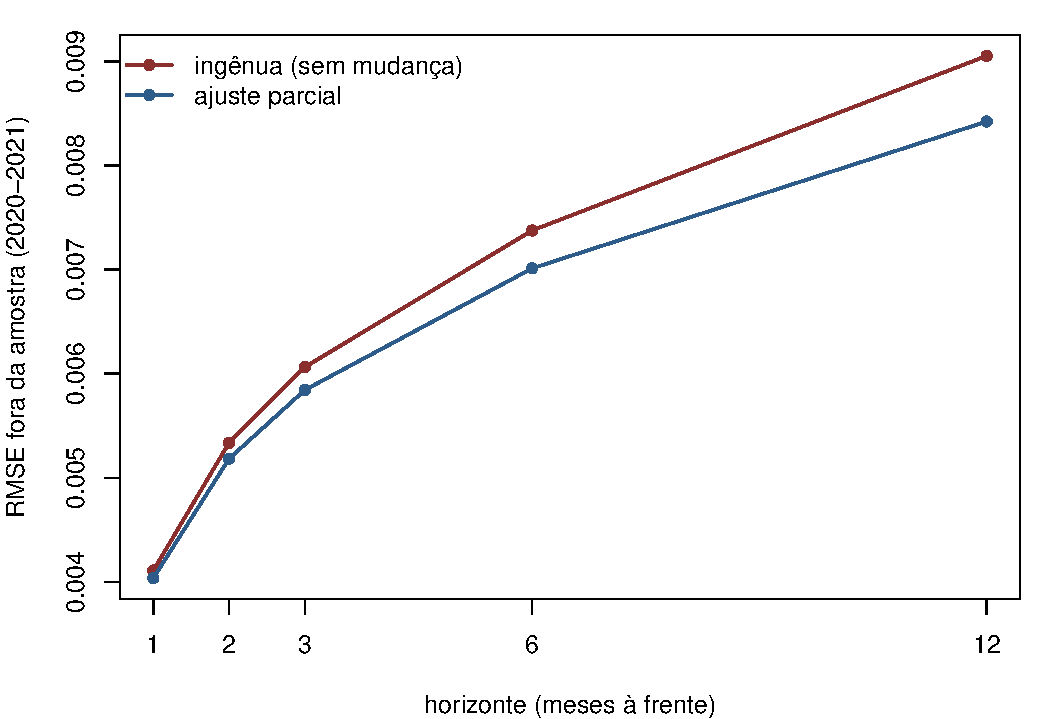
\includegraphics[width=0.75\textwidth]{fig_rmse_multihorizonte_multiativo_v2.pdf}
\caption{RMSE fora da amostra, ajuste parcial vs.\ ingênua, por horizonte --- todos os ativos e
gestoras agregados.}
\end{figure}

\aha{O ajuste parcial vence a ingênua em \textbf{100\% dos meses de teste, em todos os 5
horizontes} --- bem mais forte que o $57$--$78\%$ da Etapa 3 original (Tabela~6), porque agregar
milhões de observações por mês elimina o ruído de um único painel pequeno (23 fundos VALE3-Itaú).
A margem cresce \textbf{monotonicamente} com o horizonte ($1{,}8\%\to7{,}0\%$), sem o pico em
$h=3$-$6$ seguido de queda em $h=12$ que a versão só-VALE3 mostrava --- aqui a amostra de teste
continua grande até em $h=12$ ($1{,}4$ milhões de obs., contra só $12$ meses de VALE3-Itaú), então
o resultado não sofre da mesma instabilidade de amostra pequena. $\widehat\lambda_h$ cresce de
forma parecida à versão só-VALE3 ($0{,}075\to0{,}346$, vs.\ $0{,}195\to0{,}406$) --- mais devagar
que uma composição geométrica simples previria, mesma leitura de antes: o alvo $w^*$ também se
move no caminho, não é um decaimento a taxa constante.}

\subsubsection*{Por gestora, em todos os ativos e vários horizontes: fechando o material do robô}

\pergunta{A Tabela~22 (VALE3, $h=3$) mostrou qual gestora é mais difícil de prever fora da
amostra, mas só numa ação. O material mais completo pra decidir o desenho do robô
caça-replicantes precisa de duas coisas a mais: \textbf{todos} os ativos (não só VALE3) e
\textbf{vários horizontes} (pra saber se o ranking de ``quem é mais previsível'' é estável ou
muda dependendo de quanto tempo à frente se tenta prever).}

Mesmo esquema de sempre (equação~\eqref{eq:pa}, $\lambda_h$ único por horizonte, estimado só no
treino), agora agregado por \textbf{gestora} em vez de pooled --- reaproveita os pares $(t,t+h)$
já calculados nesta seção para $h=1$ e $h=3$, soma $h=6$ e $h=12$.

\textbf{Adendo de processo:} a primeira tentativa de montar a tabela larga (uma coluna por
horizonte) usou `gestora + nº de fundos'' como chave pra combinar os 4 horizontes --- bug real: o
nº de fundos com par $(t,t+h)$ válido \textbf{muda} de horizonte pra horizonte (quanto maior o
$h$, menos pares sobram), então usar as duas colunas juntas fragmentava cada gestora em várias
linhas parciais. Corrigido combinando só por gestora, com o nº de fundos de $h=1$ guardado à
parte como referência de cobertura.

\begin{center}\scriptsize
\begin{longtable}{@{}lrrrrr@{}}
\caption{RMSE fora da amostra por gestora, todos os 430 ativos, em 4 horizontes --- ordenado do
mais ao menos errante em $h=1$.}\\
\toprule
Gestora & Fundos ($h{=}1$) & RMSE $h{=}1$ & RMSE $h{=}3$ & RMSE $h{=}6$ & RMSE $h{=}12$ \\
\midrule
\endfirsthead
\multicolumn{6}{l}{\textit{Tabela 25 (continuação)}}\\
\toprule
Gestora & Fundos ($h{=}1$) & RMSE $h{=}1$ & RMSE $h{=}3$ & RMSE $h{=}6$ & RMSE $h{=}12$ \\
\midrule
\endhead
\midrule
\multicolumn{6}{r}{\textit{continua na próxima página}}\\
\endfoot
\bottomrule
\multicolumn{6}{@{}p{0.95\textwidth}@{}}{\footnotesize Fonte: elaboração própria
(\texttt{scripts/44\_etapa3\_multiativo\_gestora\_multihorizonte.R}).}\\
\endlastfoot
Guepardo Investimentos & 10 & $0{,}01447$ & $0{,}02392$ & $0{,}03569$ & $0{,}06177$ \\
Ibiuna Investimentos & 7 & $0{,}01331$ & $0{,}02130$ & $0{,}02491$ & $0{,}02828$ \\
AZ Quest & 22 & $0{,}01096$ & $0{,}01461$ & $0{,}01649$ & $0{,}01876$ \\
Núcleo Capital & 17 & $0{,}01045$ & $0{,}01830$ & $0{,}02490$ & $0{,}03539$ \\
Squadra Investimentos & 14 & $0{,}01007$ & $0{,}01390$ & $0{,}01681$ & $0{,}02127$ \\
Forpus Capital & 3 & $0{,}00991$ & $0{,}01430$ & $0{,}01641$ & $0{,}01661$ \\
Sharp Capital & 34 & $0{,}00813$ & $0{,}01295$ & $0{,}01709$ & $0{,}02092$ \\
Truxt Investimentos & 31 & $0{,}00812$ & $0{,}01261$ & $0{,}01596$ & $0{,}01952$ \\
Legacy Capital & 1 & $0{,}00800$ & --- & --- & --- \\
ARX Investimentos & 12 & $0{,}00792$ & $0{,}01084$ & $0{,}01262$ & $0{,}01515$ \\
Vinci Partners & 48 & $0{,}00753$ & $0{,}01053$ & $0{,}01031$ & $0{,}01272$ \\
Kinea Investimentos & 4 & $0{,}00717$ & $0{,}01160$ & $0{,}01515$ & $0{,}01543$ \\
Constellation Asset Management & 26 & $0{,}00693$ & $0{,}01377$ & $0{,}01845$ & $0{,}02775$ \\
Opportunity & 19 & $0{,}00678$ & $0{,}01052$ & $0{,}01352$ & $0{,}01594$ \\
SPX Capital & 35 & $0{,}00613$ & $0{,}00916$ & $0{,}01166$ & $0{,}01328$ \\
Atmos Capital & 28 & $0{,}00613$ & $0{,}00999$ & $0{,}01340$ & $0{,}01704$ \\
Verde Asset Management & 14 & $0{,}00600$ & $0{,}01021$ & $0{,}01293$ & $0{,}01632$ \\
Absolute Investimentos & 7 & $0{,}00589$ & $0{,}00925$ & $0{,}01216$ & $0{,}01401$ \\
Daycoval Asset Management & 5 & $0{,}00582$ & $0{,}00733$ & $0{,}00741$ & $0{,}00787$ \\
JGP & 40 & $0{,}00554$ & $0{,}00773$ & $0{,}00893$ & $0{,}01074$ \\
Kapitalo Investimentos & 22 & $0{,}00538$ & $0{,}00580$ & $0{,}00690$ & $0{,}00823$ \\
Credit Suisse & 65 & $0{,}00537$ & $0{,}00750$ & $0{,}00868$ & $0{,}00980$ \\
Bogari Capital & 14 & $0{,}00533$ & $0{,}00932$ & $0{,}01209$ & $0{,}01594$ \\
Real Investor & 5 & $0{,}00486$ & $0{,}00897$ & $0{,}01412$ & $0{,}01756$ \\
Claritas Investimentos & 10 & $0{,}00481$ & $0{,}00709$ & $0{,}00795$ & $0{,}00843$ \\
Caixa & 27 & $0{,}00461$ & $0{,}00681$ & $0{,}00888$ & $0{,}01141$ \\
Bradesco Asset Management & 281 & $0{,}00443$ & $0{,}00613$ & $0{,}00728$ & $0{,}00858$ \\
Western Asset & 26 & $0{,}00437$ & $0{,}00700$ & $0{,}00960$ & $0{,}01252$ \\
BB Asset Management & 103 & $0{,}00413$ & $0{,}00642$ & $0{,}00804$ & $0{,}00989$ \\
Occam Brasil & 26 & $0{,}00411$ & $0{,}00668$ & $0{,}00763$ & $0{,}01001$ \\
BTG Pactual & 139 & $0{,}00409$ & $0{,}00611$ & $0{,}00716$ & $0{,}00880$ \\
Santander Brasil Asset Management & 70 & $0{,}00394$ & $0{,}00551$ & $0{,}00630$ & $0{,}00735$ \\
Safra Asset Management & 137 & $0{,}00360$ & $0{,}00509$ & $0{,}00603$ & $0{,}00674$ \\
Julius Baer Family Office & 57 & $0{,}00308$ & $0{,}00416$ & $0{,}00497$ & $0{,}00570$ \\
BNP Paribas & 42 & $0{,}00300$ & $0{,}00434$ & $0{,}00527$ & $0{,}00692$ \\
XP & 87 & $0{,}00294$ & $0{,}00444$ & $0{,}00537$ & $0{,}00745$ \\
Itaú & 440 & $0{,}00264$ & $0{,}00389$ & $0{,}00473$ & $0{,}00557$ \\
Dahlia Capital & 18 & $0{,}00247$ & $0{,}00426$ & $0{,}00556$ & $0{,}00625$ \\
TNA Gestão Patrimonial & 29 & $0{,}00151$ & $0{,}00218$ & $0{,}00281$ & $0{,}00388$ \\
Gávea Investimentos & 17 & $0{,}00144$ & $0{,}00265$ & $0{,}00363$ & $0{,}00470$ \\
Plural & 1 & $0{,}00050$ & $0{,}00080$ & $0{,}00105$ & $0{,}00136$ \\
\end{longtable}
\end{center}

\aha{O ranking é \textbf{estável entre horizontes} --- correlação de Spearman entre $0{,}90$ e
$0{,}99$ em todos os pares de horizonte (a mais baixa, $0{,}90$, entre $h=1$ e $h=12$, os
extremos). Guepardo é a gestora mais difícil de prever fora da amostra em \textbf{todos os 4
horizontes}, seguida por Ibiuna e AZ Quest; Plural é a mais previsível nos 4 --- TNA Gestão
Patrimonial e Gávea Investimentos alternam entre $2^o$ e $3^o$ lugar dependendo do horizonte, mas
sempre as duas entre as três mais previsíveis. O mesmo grupo de nomes aparece nos extremos
independente de quantos meses à frente se tenta prever. Isso é uma boa notícia pro desenho do robô: a dificuldade de prever uma gestora não
é um artefato de escolher um horizonte específico, é uma característica persistente daquela
gestora. O Itaú fica perto do fim da tabela em $h=1$ (RMSE baixo, $5^o$ mais previsível de $41$)
--- consistente com o achado da Seção~\ref{sec:erro-multiativo} de que o Itaú é relativamente
``previsível'' nesse universo amplo.}

\textbf{Adendo de processo:} a Tabela~25 só mostra o RMSE do \textbf{ajuste parcial} --- não diz,
por gestora, se esse RMSE é melhor ou pior que a previsão \textbf{ingênua} (nenhuma mudança). É
uma pergunta diferente de ``quem é mais difícil de prever'' (RMSE alto pode ser só porque a
gestora se move muito, não porque o ajuste parcial falha nela especificamente). A tabela abaixo
completa essa lacuna: a \textbf{margem} de cada gestora, nos mesmos 4 horizontes.

\begin{center}\scriptsize
\begin{longtable}{@{}lrrrr@{}}
\caption{Margem do ajuste parcial sobre a ingênua ($\%$ de redução de RMSE), por gestora, 4
horizontes --- mesma ordem da Tabela~25. Negativo = ajuste parcial \textbf{pior} que a ingênua.}\\
\toprule
Gestora & Margem $h{=}1$ & Margem $h{=}3$ & Margem $h{=}6$ & Margem $h{=}12$ \\
\midrule
\endfirsthead
\multicolumn{5}{l}{\textit{Tabela 26 (continuação)}}\\
\toprule
Gestora & Margem $h{=}1$ & Margem $h{=}3$ & Margem $h{=}6$ & Margem $h{=}12$ \\
\midrule
\endhead
\midrule
\multicolumn{5}{r}{\textit{continua na próxima página}}\\
\endfoot
\bottomrule
\multicolumn{5}{@{}p{0.95\textwidth}@{}}{\footnotesize Fonte: elaboração própria
(\texttt{scripts/44\_etapa3\_multiativo\_gestora\_multihorizonte.R}).}\\
\endlastfoot
Guepardo Investimentos & $-0{,}4\%$ & $-2{,}7\%$ & $-6{,}4\%$ & $-10{,}8\%$ \\
Ibiuna Investimentos & $3{,}1\%$ & $6{,}9\%$ & $8{,}2\%$ & $14{,}9\%$ \\
AZ Quest & $3{,}2\%$ & $6{,}9\%$ & $9{,}9\%$ & $15{,}0\%$ \\
Núcleo Capital & $-1{,}6\%$ & $-3{,}0\%$ & $-2{,}8\%$ & $-6{,}0\%$ \\
Squadra Investimentos & $0{,}7\%$ & $0{,}5\%$ & $-0{,}2\%$ & $-1{,}2\%$ \\
Forpus Capital & $2{,}5\%$ & $6{,}3\%$ & $8{,}2\%$ & $11{,}8\%$ \\
Sharp Capital & $1{,}7\%$ & $5{,}0\%$ & $8{,}9\%$ & $16{,}9\%$ \\
Truxt Investimentos & $1{,}7\%$ & $3{,}7\%$ & $6{,}1\%$ & $13{,}9\%$ \\
Legacy Capital & $-11{,}2\%$ & --- & --- & --- \\
ARX Investimentos & $2{,}0\%$ & $4{,}2\%$ & $6{,}8\%$ & $7{,}5\%$ \\
Vinci Partners & $2{,}8\%$ & $6{,}1\%$ & $3{,}7\%$ & $8{,}7\%$ \\
Kinea Investimentos & $2{,}2\%$ & $4{,}1\%$ & $9{,}4\%$ & $11{,}9\%$ \\
Constellation Asset Management & $-0{,}9\%$ & $-0{,}1\%$ & $2{,}4\%$ & $3{,}4\%$ \\
Opportunity & $1{,}6\%$ & $3{,}8\%$ & $6{,}4\%$ & $9{,}3\%$ \\
SPX Capital & $2{,}8\%$ & $6{,}8\%$ & $11{,}1\%$ & $18{,}5\%$ \\
Atmos Capital & $0{,}1\%$ & $2{,}8\%$ & $5{,}0\%$ & $11{,}8\%$ \\
Verde Asset Management & $0{,}5\%$ & $1{,}6\%$ & $3{,}3\%$ & $0{,}4\%$ \\
Absolute Investimentos & $1{,}8\%$ & $4{,}1\%$ & $7{,}2\%$ & $11{,}5\%$ \\
Daycoval Asset Management & $3{,}4\%$ & $6{,}0\%$ & $8{,}4\%$ & $13{,}3\%$ \\
JGP & $2{,}2\%$ & $4{,}0\%$ & $4{,}8\%$ & $8{,}1\%$ \\
Kapitalo Investimentos & $2{,}9\%$ & $6{,}0\%$ & $7{,}5\%$ & $8{,}2\%$ \\
Credit Suisse & $2{,}5\%$ & $5{,}0\%$ & $7{,}9\%$ & $14{,}2\%$ \\
Bogari Capital & $-0{,}8\%$ & $-0{,}2\%$ & $0{,}3\%$ & $-4{,}3\%$ \\
Real Investor & $-2{,}0\%$ & $0{,}6\%$ & $1{,}7\%$ & $7{,}5\%$ \\
Claritas Investimentos & $1{,}6\%$ & $5{,}8\%$ & $10{,}6\%$ & $18{,}6\%$ \\
Caixa & $1{,}9\%$ & $4{,}3\%$ & $7{,}0\%$ & $9{,}8\%$ \\
Bradesco Asset Management & $2{,}0\%$ & $3{,}7\%$ & $4{,}6\%$ & $4{,}2\%$ \\
Western Asset & $1{,}2\%$ & $3{,}2\%$ & $5{,}4\%$ & $5{,}8\%$ \\
BB Asset Management & $1{,}1\%$ & $2{,}6\%$ & $3{,}7\%$ & $4{,}8\%$ \\
Occam Brasil & $2{,}2\%$ & $4{,}8\%$ & $7{,}8\%$ & $9{,}9\%$ \\
BTG Pactual & $1{,}8\%$ & $3{,}2\%$ & $4{,}3\%$ & $5{,}8\%$ \\
Santander Brasil Asset Management & $2{,}0\%$ & $4{,}3\%$ & $5{,}5\%$ & $7{,}3\%$ \\
Safra Asset Management & $1{,}9\%$ & $3{,}6\%$ & $6{,}1\%$ & $10{,}0\%$ \\
Julius Baer Family Office & $1{,}8\%$ & $3{,}5\%$ & $5{,}0\%$ & $7{,}1\%$ \\
BNP Paribas & $0{,}7\%$ & $0{,}7\%$ & $-0{,}6\%$ & $-1{,}1\%$ \\
XP & $-3{,}6\%$ & $-6{,}7\%$ & $-11{,}8\%$ & $-13{,}4\%$ \\
Itaú & $2{,}0\%$ & $4{,}4\%$ & $6{,}3\%$ & $8{,}1\%$ \\
Dahlia Capital & $2{,}3\%$ & $5{,}4\%$ & $8{,}3\%$ & $10{,}8\%$ \\
TNA Gestão Patrimonial & $-0{,}3\%$ & $-1{,}6\%$ & $-2{,}0\%$ & $1{,}4\%$ \\
Gávea Investimentos & $2{,}0\%$ & $4{,}1\%$ & $8{,}0\%$ & $10{,}6\%$ \\
Plural & $-3{,}3\%$ & $-4{,}9\%$ & $-4{,}2\%$ & $-8{,}1\%$ \\
\end{longtable}
\end{center}

\aha{Quatro gestoras --- \textbf{Guepardo, Núcleo Capital, XP e Plural} --- têm margem
\textbf{negativa nos 4 horizontes}: pra elas, o ajuste parcial é \textbf{pior} que simplesmente
assumir que nada muda. Isso é uma distinção importante que a Tabela~25 sozinha não mostrava ---
``difícil de prever'' (RMSE alto) não é o mesmo que ``a fórmula atrapalha'' (margem negativa). A
Guepardo ilustra os dois problemas ao mesmo tempo: RMSE mais alto \emph{e} margem cada vez mais
negativa com o horizonte ($-0{,}4\%\to-10{,}8\%$) --- as apostas concentradas e de curto prazo que
já vimos (o salto de $13\%$ pra $80\%$ em VALE3) tornam qualquer ajuste baseado em $\lambda$
enganoso pra essa gestora especificamente. Já a \textbf{Plural} é o oposto: RMSE \textbf{baixíssimo}
(a mais previsível de todas), mas ainda assim margem negativa --- o motivo aqui não é volatilidade,
é o contrário: as posições da Plural quase não mudam (só $1$ fundo, série muito estável), então a
ingênua (zero mudança) já acerta quase tudo sozinha, e qualquer ajuste pelo $\lambda$ introduz
ruído onde não tinha erro pra corrigir. Pro robô: essas $4$ gestoras merecem tratamento à parte ---
não são bons alvos pra um modelo baseado em ajuste parcial, seja porque decidem rápido demais
(Guepardo, Núcleo Capital, XP) ou porque simplesmente não se mexem (Plural).}

% ======================================================================
\FloatBarrier
\section{Resumo}

\begin{enumerate}[topsep=2pt,itemsep=3pt]
\item \textbf{Etapa 1, equações~\eqref{eq:cs}--\eqref{eq:logit}:} $\theta_t$ mês a mês, cinco
características (agora incluindo beta do fundo), todas predeterminadas ($t-1$). Com o beta do
fundo na conta, tamanho e cotistas ficam bem mais fracos em magnitude de $t$, mas o APE (efeito
marginal médio, pontos percentuais) de ambos continua *** significativo; fundo de cotas e beta do
fundo continuam com a força quase intacta. Pseudo-$R^2$ médio $0{,}614$ (era $0{,}164$). Custo:
cobertura cai para 59 meses (fev/2017 em diante).
\item \textbf{Etapa 2, equação~\eqref{eq:pa}:} $\widehat\lambda=0{,}153$ (era $0{,}098$) --- um
alvo mais preciso atenua menos o coeficiente. Erro $u$ com comportamento parecido ao da versão
anterior.
\item \textbf{Etapa 3:} $\lambda$ treinado em 2017--2019 vence a ingênua fora da amostra
(2020--2021) em RMSE, por margem pequena mas consistente ($1{,}5\%$; vence em $61\%$ dos meses
de teste) --- resultado qualitativamente igual ao da versão anterior. Flexibilizando para outros
horizontes ($h=2,3,6,12$ meses), a vantagem se mantém nos 5 horizontes testados, com margem
maior em $h=3$-$6$ ($\approx4\%$) e quase sumindo em $h=12$ (amostra de teste pequena, só 12
meses).
\item \textbf{Extensão de gestoras (Seção~\ref{sec:gestoras}):} o padrão da Etapa 1 generaliza
para além do Itaú --- $2.820$ fundos, $41$ grupos de gestora, o APE das cinco características
sobrevive quase intacto ao entrar o efeito fixo de gestora (pseudo-$R^2$ $0{,}604\to0{,}696$);
tamanho fica bem mais fraco no coeficiente bruto (log-odds), mas o APE continua significativo.
Gestoras de varejo/plataforma carregam mais VALE3 que o Itaú equivalente; boutiques de gestão
concentrada carregam bem menos.
\item \textbf{Extensão de todas as ações (Seção~\ref{sec:multiativo}):} mesmo universo de
fundos/gestoras, agora testado em $501$ ativos ($13.938$ células ativo-mês convergidas). O beta
do fundo é a característica que mais generaliza ($96$--$97\%$ dos ativos com o mesmo sinal de
VALE3, pelo coeficiente e pelo APE) e a única que sobrevive robusta numa regressão pooled com
efeito-fixo de ativo e mês ($t=28{,}6$); tamanho, cotistas e fluxo generalizam bem mais fraco do
que a v1 havia encontrado (tamanho e FIC, pelo APE, generalizam no nível do acaso). Estendendo
o erro dessa mesma regressão para todas as ações (Seção~\ref{sec:erro-multiativo}, $8.251.936$
obs.), $36$ das $41$ gestoras têm viés significativo (mas em geral pequeno) e a Guepardo tem o
viés mais positivo e, disparada, a maior dispersão (mais que o dobro da segunda colocada); viés e
dispersão andam juntos (correlação $0{,}88$) --- material que vai orientar o desenho do robô
caça-replicantes, decisão
ainda em aberto. Ainda restrito a VALE3 no ajuste parcial/in-out-of-sample desta rodada.
\item \textbf{Gestora de volta ao painel completo, via pooled com 3 efeitos-fixos (Seção 6.1):}
uma única regressão com efeito-fixo de ativo, mês \emph{e} gestora simultâneos --- a primeira vez que o
coeficiente por gestora é estimado no painel completo ($430$ ativos), não só VALE3. Tamanho e
fundo de cotas deixam de ser significativos (o efeito-fixo de gestora absorve boa parte do que
pareciam captar); beta do fundo não se move ($t=29{,}0$). A ordem das gestoras quase se
\textbf{inverte} em relação à Seção~\ref{sec:gestoras}: boutiques de gestão concentrada (Guepardo,
Núcleo Capital, Bogari), que carregavam \emph{menos} VALE3 que o Itaú, têm o efeito-fixo mais alto
olhando a carteira inteira --- montam posições maiores em geral, mas evitam especificamente o
blue chip mega-cap. Essa ordenação bate com o viés do erro por gestora (Seção~\ref{sec:erro-multiativo}),
duas metodologias independentes chegando à mesma conclusão.
\item \textbf{Etapa 3 generalizada (Seção~\ref{sec:etapa3-multiativo}):} o mesmo ajuste parcial
fora da amostra testado para todos os fundos, gestoras e ativos, reaproveitando o alvo $w^*$ já
calculado na Seção~\ref{sec:multiativo}. Em VALE3 ($h=3$), a Vinci Partners é a gestora mais
difícil de prever fora da amostra (cobertura ampla, não é artefato de poucos fundos); o fundo mais
errante tem uma aposta real e concentrada de curtíssimo prazo (13\%$\to$80\%$\to$11\% em 3 meses,
AUM estável, não é resgate). Generalizando para todos os ativos ($h=1$, com o mesmo filtro de
posição-poeira das seções anteriores): $89{,}6\%$ dos $48$ ativos elegíveis têm o ajuste parcial
vencendo a ingênua fora da amostra, mediana de $1{,}85\%$ --- mais forte que o $1{,}5\%$ da Etapa
3 original, um sinal de que a vantagem do ajuste parcial não é uma particularidade de VALE3.
\item \textbf{Flexibilização de lags, todos os ativos:} o teste multi-horizonte ($h=1,2,3,6,12$)
da Seção~4.2, generalizado para o painel multiativo inteiro (\emph{pooled}, não fundo-ativo por
vez). O ajuste parcial vence a ingênua em $100\%$ dos meses de teste, em \textbf{todos} os $5$
horizontes --- mais forte e mais estável que o $57$--$78\%$ da versão só-VALE3, porque agregar
milhões de observações por mês elimina o ruído de um painel pequeno. A margem cresce
monotonicamente com o horizonte ($1{,}8\%\to7{,}0\%$), sem o pico seguido de queda que a versão
só-VALE3 mostrava em $h=12$ (aqui a amostra de teste continua grande, $1{,}4$ milhões de obs.).
\item \textbf{Erro fora da amostra por gestora, todos os ativos, 4 horizontes:} fecha o material
completo pro robô caça-replicantes --- RMSE fora da amostra por gestora ($h=1,3,6,12$), não mais
restrito a VALE3. O ranking de quem é mais/menos previsível é \textbf{estável entre horizontes}
(correlação de Spearman entre $0{,}90$ e $0{,}99$): Guepardo é a mais difícil de prever nos $4$
horizontes; Plural, a mais previsível nos $4$. O Itaú fica entre as $5$ mais previsíveis de $41$.
Comparando com a ingênua, $4$ gestoras (Guepardo, Núcleo Capital, XP, Plural) têm margem
\textbf{negativa} nos $4$ horizontes --- pra elas o ajuste parcial \emph{piora} a previsão, por
motivos opostos: Guepardo/Núcleo Capital/XP decidem rápido demais pro modelo captar; a Plural
simplesmente não se mexe, e a ingênua já acerta sozinha.
\end{enumerate}

Nenhuma dessas conclusões depende de Newey--West, cluster, Kalman, variável instrumental ou
teste de Diebold--Mariano --- o preço da simplicidade é não corrigir os vieses conhecidos do
MQO direto no ajuste parcial, que a versão anterior do projeto documentou e tentou corrigir.
Fica registrado como decisão consciente, não como descuido.

\end{document}
